%%%%%%%%%%%% Procesadores CMP: usando la vectorización y la paralelización  %%%%%%%%%%%%

\begin{center}
	\rule{15cm}{0pt} \\
	{\fboxrule=4pt \fbox{\fboxrule=1pt
		\fbox{\large{\bfseries Procesadores CMP: usando la vectorización y la paralelización}}}} \\
	\addcontentsline{toc}{chapter}{2. Procesadores CMP: usando la vectorización y la paralelización}
	\setcounter{chapter}{2}
	\setcounter{section}{0}
	\rule{15cm}{0pt} \\
\end{center}

%%%%%%%%%%%%%%%%%%%%%% Procesadores CMP: usando la vectorización y la paralelización - EJERCICIO 1 %%%%%%%%%%%%%%%%%%%%%%
\section{Ejercicio 1}
\subsection{Enunciado}
\begin{ejer}
    \textbf{1.-} En el subdirectorio \texttt{vectorización} hay un pequeño programa que tiene 6 bucles.
    \begin{itemize}
        \item Para cada uno de los bucles del programa, identifica las dependencias entre iteraciones que tiene
    y explica cómo afectarían a una posible vectorización automática.
        \item Utiliza el \texttt{Makefile} incluido para compilar el programa con el compilador \texttt{ICC} y generar
    el informe de optimización. Para cada bucle mencionado en el informe, explica por qué ha sido vectorizado o por qué no 
    se ha podido vectorizar. En especial, para los bucles en los que se hubieran identificado dependencias entre iteraciones
     en el punto anterior:
        \begin{itemize}
            \item Explica en caso de que haya sido vectorizado qué transformaciones ha aplicado automáticamente el compilador.
            \item Y en caso de que no haya sido vectorizado, indica si crees que existe alguna transformación manual posible para
            que se pudiera vectorizar.
        \end{itemize}
    \end{itemize}
\end{ejer}

\subsection{Identificación dependencias}
\par Solo analizo los bucles internos, porque la vectorización consiste en ejecutar en paralelo las operaciones matemáticas realizadas en 
los bucles internos de aplicaciones de código científico.
\par Hay varias estrategias para usar código vectorial en los programas, en este caso dejo que el compilador 
vectorice automáticamente.


\subsubsection{\textbf{1ºBucle:}}
\par El primer bucle es \texttt{while(difference / (state.height * state.width) > tolerance)}. Se podría paralelizar creando una rama master y añadiendo un pragma de tipo
\texttt{task} que comparte la variable \texttt{iterations} antes del \texttt{if(verbose)} porque la ejecución de la siguiente iteración no depende de esto.
Además, dentro de esta \texttt{task} se necesita un pragma \texttt{atomic}, porque solo un hilo puede modificar a la vez esa variable global. Esta
implementación, mostrada en el código siguiente, no ayuda mucho en el rendimiento de la aplicación y la mejora es despreciable e incluso en 
algunos casos es peor como se indica en todas las tablas y gráficas.
%%% TABLA DE TIEMPOS E IMÁGENES %%%
\begin{figure}[H]
    \centering
    \begin{subfigure}{0.4\textwidth}
        \begin{adjustbox}{width=\textwidth} 
        \begin{tabular}{|c|c|c|c|c|}
            \hline
            \rowcolor{azul} \multicolumn{2}{|c|}{}&\multicolumn{3}{c|}{\textbf{Compiler}} \\ \hline
            \rowcolor{azul} \multicolumn{2}{|c|}{}&\texttt{clang}&\texttt{gcc}&\texttt{icc}\\ \hline
            \rowcolor{azul} \textbf{Testing size} & \textbf{Threads}&\multicolumn{3}{c|}{\textbf{Average time (s)}} \\ \hline
            \multirow{8}{1cm}{\textbf{01-small}} & 1 & \(1.58\pm{0.03}\) & \(0.32\pm{0.01}\) & \(1.00\pm{0.01}\) \\ \cline{2-5}
            & 2 & \(1.58\pm{0.03}\) & \(0.32\pm{0.01}\) & \(1.02\pm{0.01}\) \\ \cline{2-5}
            & 3 & \(1.60\pm{0.03}\) & \(0.33\pm{0.01}\) & \(1.02\pm{0.01}\) \\ \cline{2-5}
            & 4 & \(1.62\pm{0.01}\) & \(0.33\pm{0.01}\) & \(1.08\pm{0.04}\) \\ \cline{2-5}
            & 5 & \(1.62\pm{0.01}\) & \(0.33\pm{0.01}\) & \(1.05\pm{0.01}\) \\ \cline{2-5}
            & 6 & \(1.72\pm{0.01}\) & \(0.46\pm{0.01}\) & \(1.41\pm{0.35}\) \\ \cline{2-5}
            & 7 & \(1.99\pm{0.01}\) & \(0.47\pm{0.01}\) & \(1.44\pm{0.32}\) \\ \cline{2-5}
            & 8 & \(1.85\pm{0.01}\) & \(0.47\pm{0.02}\) & \(1.77\pm{0.02}\) \\ \hline
        \end{tabular}
        \end{adjustbox}
    \end{subfigure}
    \hfill
    \begin{subfigure}{0.5\textwidth}
        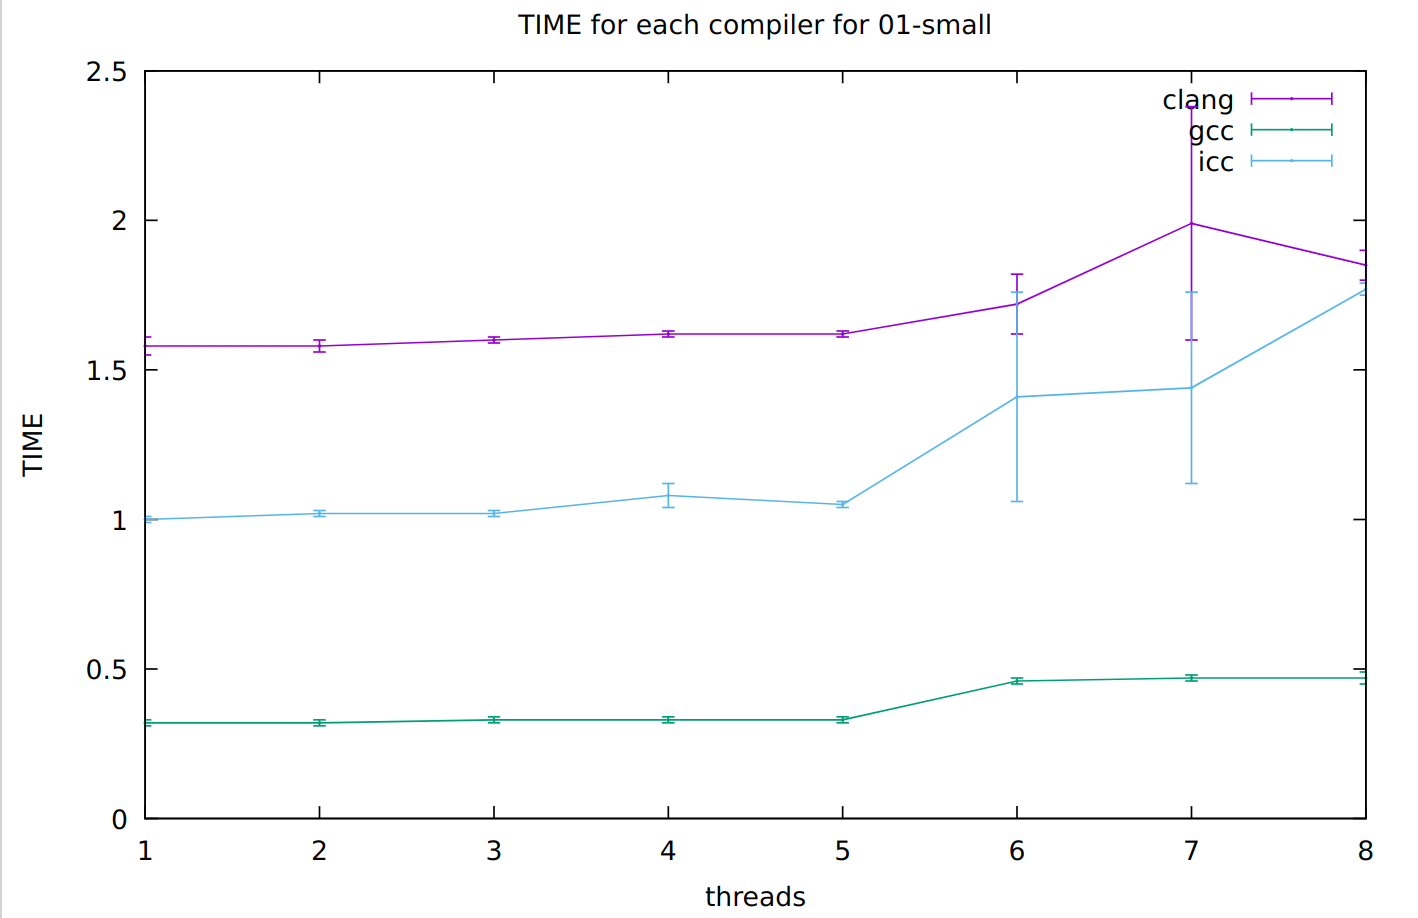
\includegraphics[width=\textwidth]{bucle1=01-small}
    \end{subfigure}
    \caption{\underline{1º Bucle, tamaño pequeño}: Tiempos de ejecución vs nº de hilos}
    \label{fig:bucle1=01-small}
\end{figure}
\newpage

\subsubsection{\textbf{heat.cpp}}
\begin{listing}[firstnumber=20]
    @@ -21,28 +21,36 @@
    void solve(Matrix<double>& state, double tolerance, int& iterations, double& last_difference) {
    Matrix<double> next_state = state;
    iterations = 0;
    double difference;
  + #pragma omp parallel
  + {
  + #pragma omp master
    do {
        difference = 0;
        for (size_t i = 1; i < state.height - 1; ++i) {
            for (size_t j = 1; j < state.width - 1; ++j) {
                next_state[i][j] = (state[i][j]
                                + state[i + 1][j]  
                                + state[i - 1][j]  
                                + state[i][j + 1]  
                                + state[i][j - 1]) / 5;
                difference = difference 
                             + abs(next_state[i][j]-state[i][j]);
            }
        }

        state.swap_data(next_state);

  + #pragma omp task shared(iterations)
  + {    
        if (verbose) {
            cout << "Iteration " << iterations << ":" << endl;
            printf_matrix("%7.3f", state);
            cout << "Difference: " << difference << endl;
        }
  + #pragma omp atomic
        ++iterations;
  + }
    } while (difference / (state.height * state.width) > tolerance);
    last_difference = difference / (state.height * state.width);
  + }
    }
\end{listing}


%%% TABLA DE TIEMPOS E IMÁGENES %%%
\begin{figure}[H]
    \centering
    \begin{subfigure}{0.4\textwidth}
        \begin{adjustbox}{width=\textwidth} 
        \begin{tabular}{|c|c|c|c|c|}
            \hline
            \rowcolor{azul} \multicolumn{2}{|c|}{}&\multicolumn{3}{c|}{\textbf{Compiler}} \\ \hline
            \rowcolor{azul} \multicolumn{2}{|c|}{}&\texttt{clang}&\texttt{gcc}&\texttt{icc}\\ \hline
            \rowcolor{azul} \textbf{Testing size} & \textbf{Threads}&\multicolumn{3}{c|}{\textbf{Average time (s)}} \\ \hline
            \multirow{8}{2.5cm}{\textbf{02-medium}} & 1 & \(4.83\pm{0.42}\) & \(0.89\pm{0.04}\) & \(2.88\pm{0.04}\) \\ \cline{2-5}
            & 2 & \(4.73\pm{0.24}\) & \(0.91\pm{0.04}\) & \(2.94\pm{0.04}\) \\ \cline{2-5}
            & 3 & \(4.57\pm{0.07}\) & \(0.90\pm{0.03}\) & \(3.22\pm{0.22}\) \\ \cline{2-5}
            & 4 & \(5.19\pm{0.57}\) & \(0.93\pm{0.04}\) & \(3.19\pm{0.21}\) \\ \cline{2-5}
            & 5 & \(4.63\pm{0.04}\) & \(1.28\pm{0.03}\) & \(3.16\pm{0.15}\) \\ \cline{2-5}
            & 6 & \(4.63\pm{0.03}\) & \(1.27\pm{0.03}\) & \(4.20\pm{0.86}\) \\ \cline{2-5}
            & 7 & \(4.64\pm{0.03}\) & \(1.27\pm{0.03}\) & \(4.83\pm{0.24}\) \\ \cline{2-5}
            & 8 & \(5.41\pm{0.08}\) & \(1.20\pm{0.04}\) & \(5.17\pm{0.10}\) \\ \hline
        \end{tabular}
        \end{adjustbox}
    \end{subfigure}
    \hfill
    \begin{subfigure}{0.5\textwidth}
        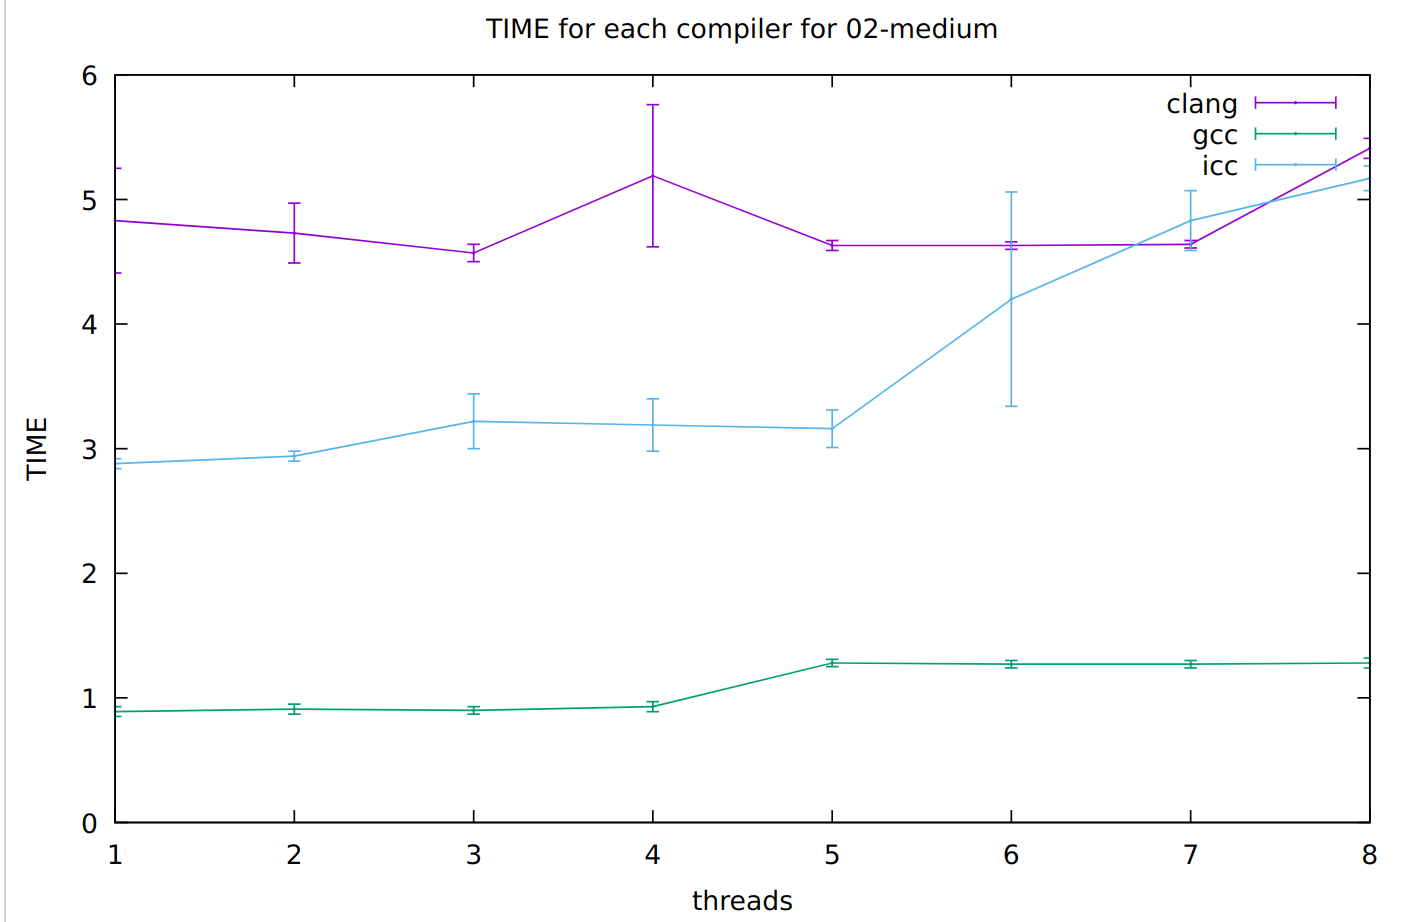
\includegraphics[width=\textwidth]{bucle1=02-medium}
    \end{subfigure}
    \caption{\underline{1º Bucle, tamaño mediano}: Tiempos de ejecución vs nº de hilos}
    \label{bucle1=02-medium}
\end{figure}

%%% TABLA DE TIEMPOS E IMÁGENES %%%
\begin{figure}[H]
    \centering
    \begin{subfigure}{0.4\textwidth}
        \begin{adjustbox}{width=\textwidth} 
        \begin{tabular}{|c|c|c|c|c|}
            \hline
            \rowcolor{azul} \multicolumn{2}{|c|}{}&\multicolumn{3}{c|}{\textbf{Compiler}} \\ \hline
            \rowcolor{azul} \multicolumn{2}{|c|}{}&\texttt{clang}&\texttt{gcc}&\texttt{icc}\\ \hline
            \rowcolor{azul} \textbf{Testing size} & \textbf{Threads}&\multicolumn{3}{c|}{\textbf{Average time (s)}} \\ \hline
            \multirow{8}{1cm}{\textbf{03-large}} & 1 & \(7.58\pm{0.01}\) & \(1.54\pm{0.11}\) & \(4.97\pm{0.13}\) \\ \cline{2-5}
            & 2 & \(7.69\pm{0.05}\) & \(1.55\pm{0.07}\) & \(5.11\pm{0.16}\) \\ \cline{2-5}
            & 3 & \(7.83\pm{0.01}\) & \(1.56\pm{0.08}\) & \(5.20\pm{0.21}\) \\ \cline{2-5}
            & 4 & \(7.87\pm{0.06}\) & \(1.61\pm{0.09}\) & \(5.23\pm{0.16}\) \\ \cline{2-5}
            & 5 & \(7.90\pm{0.03}\) & \(2.19\pm{0.05}\) & \(5.23\pm{0.18}\) \\ \cline{2-5}
            & 6 & \(7.87\pm{0.05}\) & \(2.17\pm{0.05}\) & \(5.20\pm{0.14}\) \\ \cline{2-5}
            & 7 & \(8.86\pm{0.01}\) & \(2.16\pm{0.06}\) & \(8.78\pm{0.18}\) \\ \cline{2-5}
            & 8 & \(8.85\pm{0.03}\) & \(2.15\pm{0.03}\) & \(8.76\pm{0.15}\) \\ \hline
        \end{tabular}
        \end{adjustbox}
    \end{subfigure}
    \hfill
    \begin{subfigure}{0.5\textwidth}
        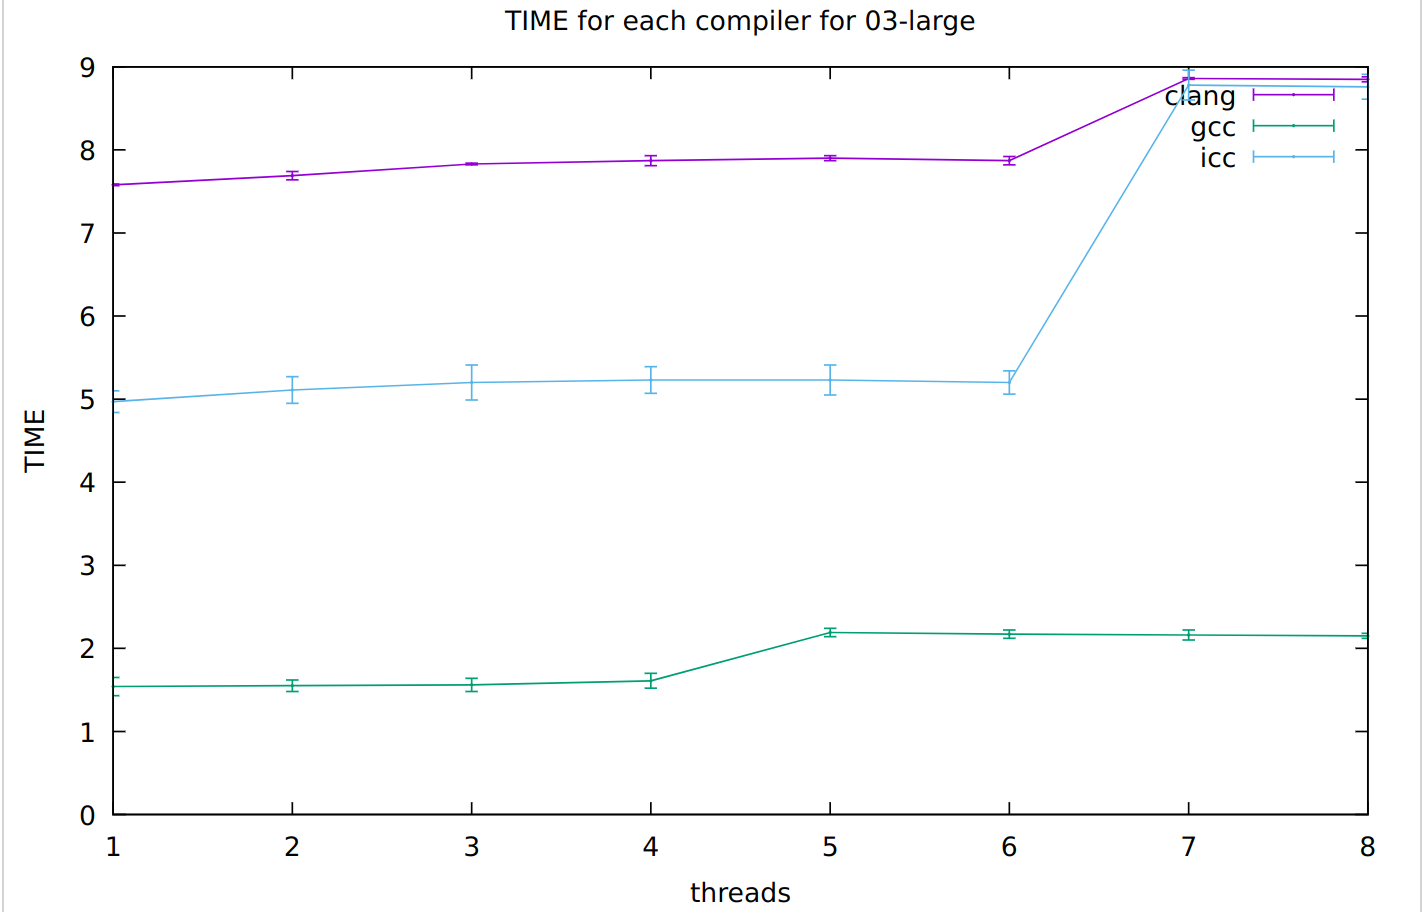
\includegraphics[width=\textwidth]{bucle1=03-large}
    \end{subfigure}
    \caption{\underline{1º Bucle, tamaño largo}: Tiempos de ejecución vs nº de hilos}
    \label{bucle1=03-large}
\end{figure}

\subsubsection{\textbf{2ºBucle:}}

\par El segundo es el bucle exterior \texttt{for (size\_t i = 1; i < state.height - 1; ++i)}, es el mejor candidato para paralelizar, hay que añadir un
pragma \texttt{\#pragma omp parallel for reduction (max:difference)} para que ejecute las instrucciones en paralelo pero tenga en cuenta la
instrucción max que no deben de ejecutarla dos hilos a la vez.

%%% TABLA DE TIEMPOS E IMÁGENES %%%
\begin{figure}[H]
    \centering
    \begin{subfigure}{0.4\textwidth}
        \begin{adjustbox}{width=\textwidth} 
        \begin{tabular}{|c|c|c|c|c|}
            \hline
            \rowcolor{azul} \multicolumn{2}{|c|}{}&\multicolumn{3}{c|}{\textbf{Compiler}} \\ \hline
            \rowcolor{azul} \multicolumn{2}{|c|}{}&\texttt{clang}&\texttt{gcc}&\texttt{icc}\\ \hline
            \rowcolor{azul} \textbf{Testing size} & \textbf{Threads}&\multicolumn{3}{c|}{\textbf{Average time (s)}} \\ \hline
            \multirow{8}{1cm}{\textbf{01-small}} & 1 & \(1.53\pm{0.00}\) & \(0.36\pm{0.00}\) & \(1.01\pm{0.01}\) \\ \cline{2-5}
            & 2 & \(0.81\pm{0.02}\) & \(0.18\pm{0.01}\) & \(0.53\pm{0.01}\) \\ \cline{2-5}
            & 3 & \(0.54\pm{0.00}\) & \(0.13\pm{0.01}\) & \(0.37\pm{0.00}\) \\ \cline{2-5}
            & 4 & \(0.42\pm{0.00}\) & \(0.12\pm{0.03}\) & \(0.34\pm{0.05}\) \\ \cline{2-5}
            & 5 & \(0.41\pm{0.01}\) & \(0.14\pm{0.01}\) & \(0.45\pm{0.01}\) \\ \cline{2-5}
            & 6 & \(0.35\pm{0.01}\) & \(0.13\pm{0.02}\) & \(0.40\pm{0.03}\) \\ \cline{2-5}
            & 7 & \(0.31\pm{0.01}\) & \(0.11\pm{0.00}\) & \(0.33\pm{0.01}\) \\ \cline{2-5}
            & 8 & \(0.29\pm{0.01}\) & \(0.11\pm{0.00}\) & \(0.33\pm{0.02}\) \\ \hline
        \end{tabular}
        \end{adjustbox}
    \end{subfigure}
    \hfill
    \begin{subfigure}{0.5\textwidth}
        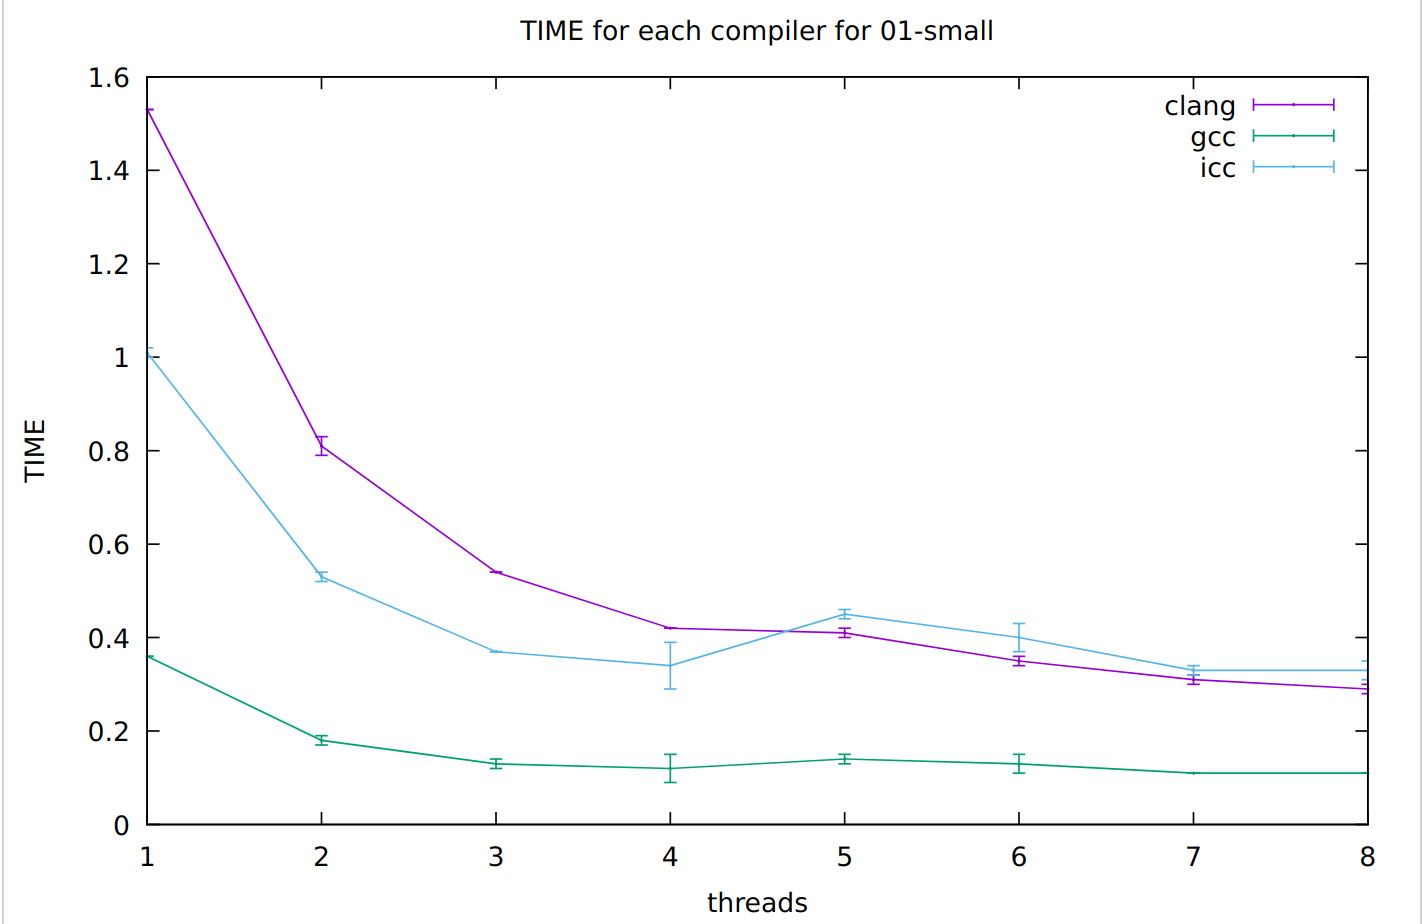
\includegraphics[width=\textwidth]{bucle2=01-small}
    \end{subfigure}
    \caption{\underline{Tamaño pequeño}: Tiempos de ejecución vs nº de hilos}
    \label{fig:bucle2=01-small}
\end{figure}

%%% TABLA DE TIEMPOS E IMÁGENES %%%
\begin{figure}[H]
    \centering
    \begin{subfigure}{0.4\textwidth}
        \begin{adjustbox}{width=\textwidth} 
        \begin{tabular}{|c|c|c|c|c|}
            \hline
            \rowcolor{azul} \multicolumn{2}{|c|}{}&\multicolumn{3}{c|}{\textbf{Compiler}} \\ \hline
            \rowcolor{azul} \multicolumn{2}{|c|}{}&\texttt{clang}&\texttt{gcc}&\texttt{icc}\\ \hline
            \rowcolor{azul} \textbf{Testing size} & \textbf{Threads}&\multicolumn{3}{c|}{\textbf{Average time (s)}} \\ \hline
            \multirow{8}{2.5cm}{\textbf{02-medium}} & 1 & \(4.45\pm{0.03}\) & \(0.89\pm{0.03}\) & \(2.90\pm{0.03}\) \\ \cline{2-5}
            & 2 & \(2.31\pm{0.05}\) & \(0.47\pm{0.02}\) & \(3.37\pm{0.06}\) \\ \cline{2-5}
            & 3 & \(1.52\pm{0.00}\) & \(0.33\pm{0.02}\) & \(2.93\pm{0.05}\) \\ \cline{2-5}
            & 4 & \(1.20\pm{0.03}\) & \(0.30\pm{0.06}\) & \(2.97\pm{0.03}\) \\ \cline{2-5}
            & 5 & \(1.16\pm{0.04}\) & \(0.37\pm{0.02}\) & \(2.96\pm{0.02}\) \\ \cline{2-5}
            & 6 & \(0.97\pm{0.03}\) & \(0.31\pm{0.01}\) & \(2.96\pm{0.07}\) \\ \cline{2-5}
            & 7 & \(0.87\pm{0.05}\) & \(0.27\pm{0.01}\) & \(2.93\pm{0.02}\) \\ \cline{2-5}
            & 8 & \(0.77\pm{0.03}\) & \(0.25\pm{0.01}\) & \(2.92\pm{0.01}\) \\ \hline
        \end{tabular}
        \end{adjustbox}
    \end{subfigure}
    \hfill
    \begin{subfigure}{0.5\textwidth}
        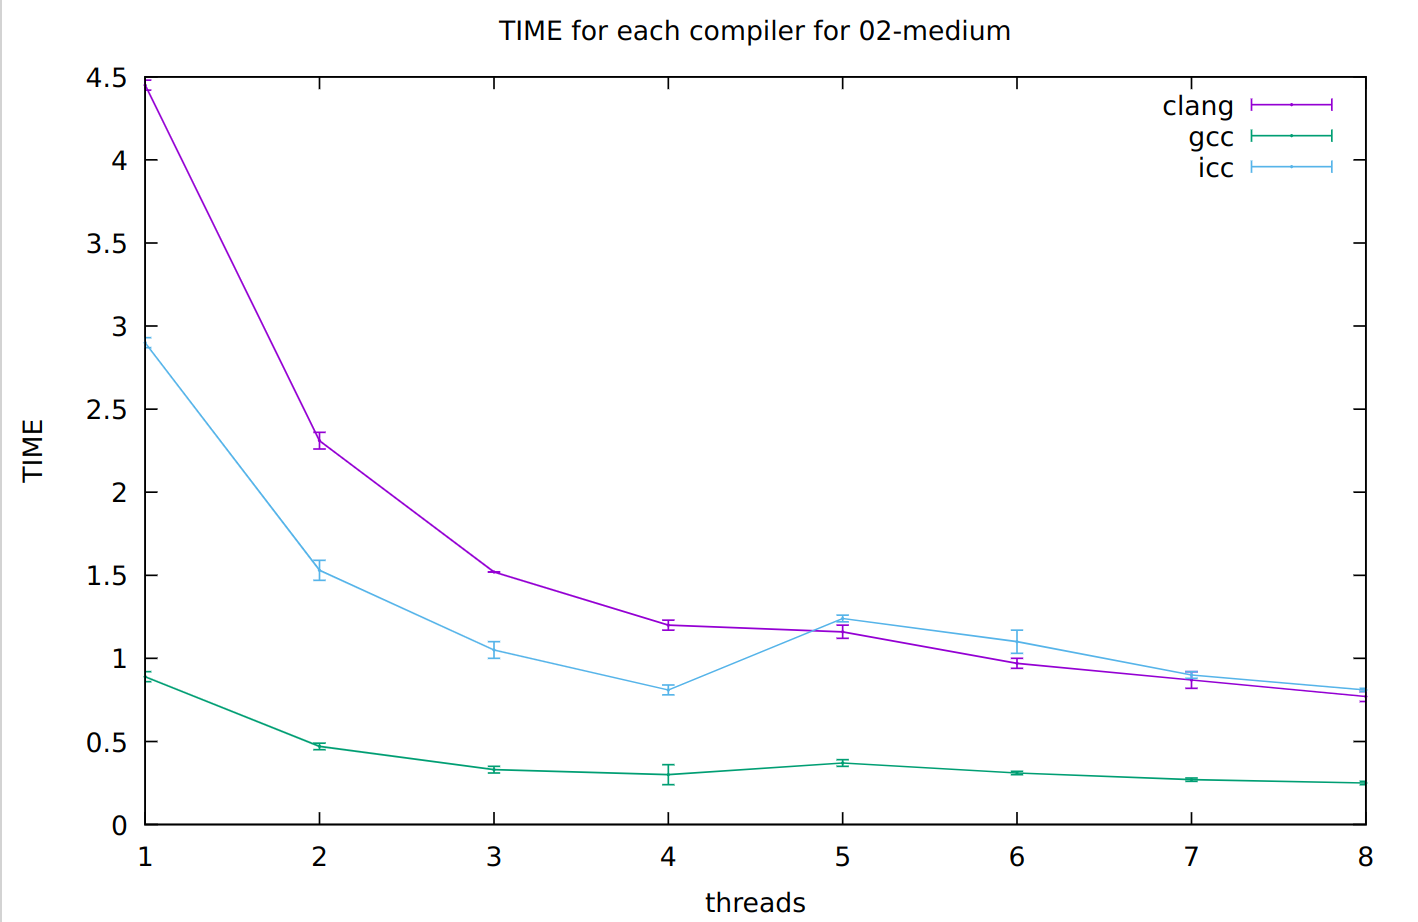
\includegraphics[width=\textwidth]{bucle2=02-medium}
    \end{subfigure}
    \caption{\underline{Tamaño mediano}: Tiempos de ejecución vs nº de hilos}
    \label{bucle2=02-medium}
\end{figure}

%%% TABLA DE TIEMPOS E IMÁGENES %%%
\begin{figure}[H]
    \centering
    \begin{subfigure}{0.4\textwidth}
        \begin{adjustbox}{width=\textwidth} 
        \begin{tabular}{|c|c|c|c|c|}
            \hline
            \rowcolor{azul} \multicolumn{2}{|c|}{}&\multicolumn{3}{c|}{\textbf{Compiler}} \\ \hline
            \rowcolor{azul} \multicolumn{2}{|c|}{}&\texttt{clang}&\texttt{gcc}&\texttt{icc}\\ \hline
            \rowcolor{azul} \textbf{Testing size} & \textbf{Threads}&\multicolumn{3}{c|}{\textbf{Average time (s)}} \\ \hline
            \multirow{8}{1cm}{\textbf{03-large}} & 1 & \(7.62\pm{0.15}\) & \(1.56\pm{0.07}\) & \(5.00\pm{0.12}\) \\ \cline{2-5}
            & 2 & \(3.93\pm{0.05}\) & \(0.80\pm{0.04}\) & \(2.63\pm{0.11}\) \\ \cline{2-5}
            & 3 & \(2.65\pm{0.02}\) & \(0.55\pm{0.04}\) & \(1.85\pm{0.15}\) \\ \cline{2-5}
            & 4 & \(2.02\pm{0.02}\) & \(0.42\pm{0.02}\) & \(1.37\pm{0.05}\) \\ \cline{2-5}
            & 5 & \(1.97\pm{0.12}\) & \(0.60\pm{0.03}\) & \(2.10\pm{0.02}\) \\ \cline{2-5}
            & 6 & \(1.67\pm{0.09}\) & \(0.51\pm{0.02}\) & \(1.78\pm{0.05}\) \\ \cline{2-5}
            & 7 & \(1.43\pm{0.07}\) & \(0.47\pm{0.04}\) & \(1.51\pm{0.02}\) \\ \cline{2-5}
            & 8 & \(1.28\pm{0.06}\) & \(0.41\pm{0.02}\) & \(1.40\pm{0.05}\) \\ \hline
        \end{tabular}
        \end{adjustbox}
    \end{subfigure}
    \hfill
    \begin{subfigure}{0.5\textwidth}
        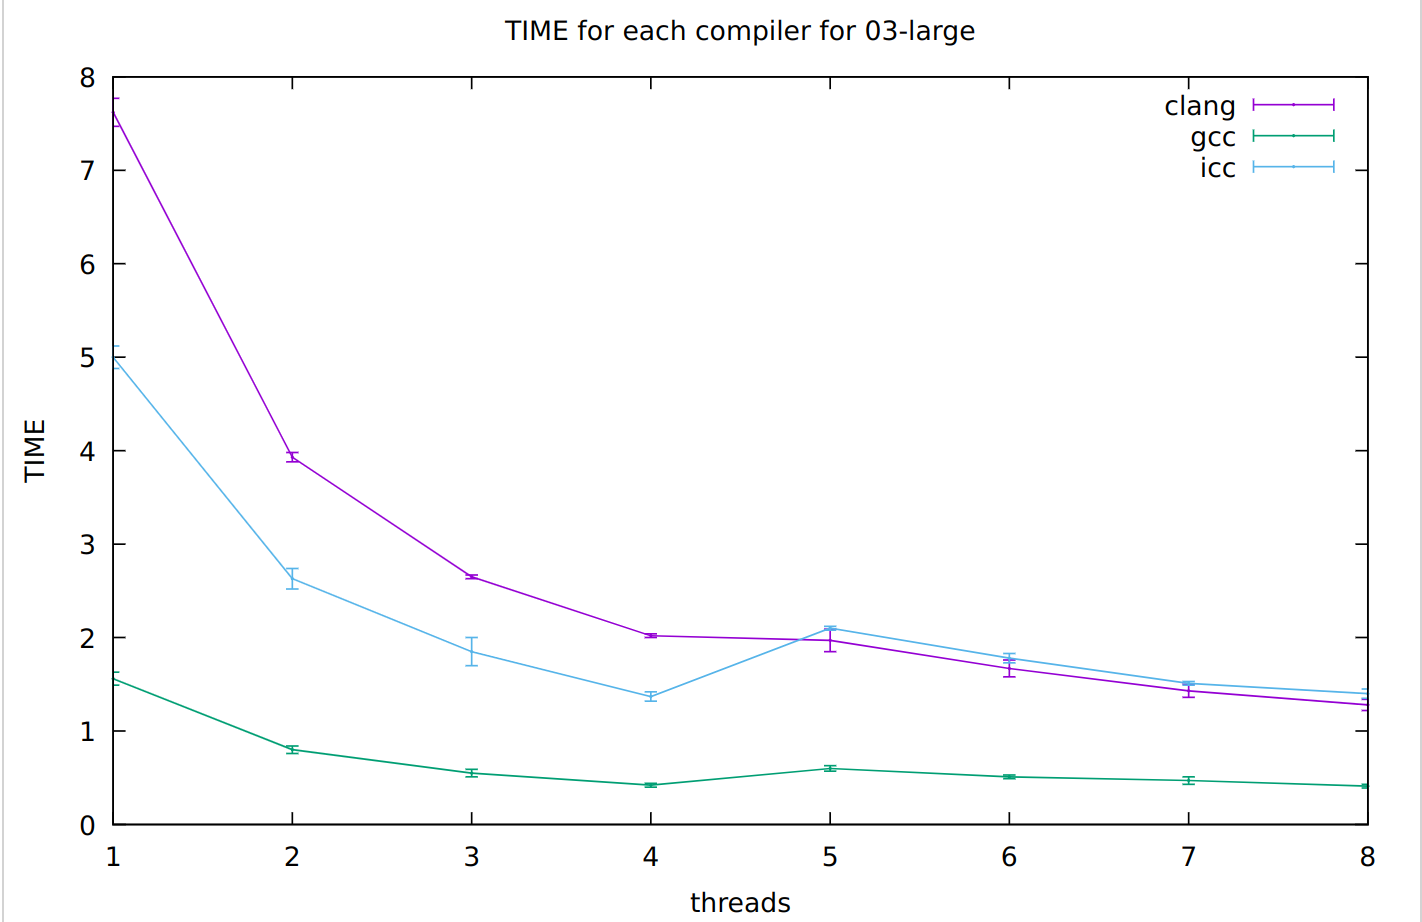
\includegraphics[width=\textwidth]{bucle2=03-large}
    \end{subfigure}
    \caption{\underline{Tamaño largo}: Tiempos de ejecución vs nº de hilos}
    \label{bucle2=03-large}
\end{figure}
\subsubsection{\textbf{3ºBucle:}}
\begin{listing}
    @@ -20,3 +20,4 @@
\end{listing}
\subsubsection{\textbf{4ºBucle:}}
\begin{listing}[firstnumber=31]
    @@ -32,3 +32,3 @@
    for (int i = 0; i < arrays_size; ++i) {
      C[i] = A[i] + 2 * B[i];
    }
\end{listing}
\par No hace falta analizar la ejecución desarrollada del bucle porque mirando el código se puede decir a simple vista que no hay
\textbf{ninguna dependencia} entre iteraciones, porque en cada iteración solo se necesita los valores que se leen y procesan en ella misma.
El compilador podrá vectorizar automáticamente este bucle sin ninguna modificación.
\subsubsection{\textbf{5ºBucle:}}
\begin{listing}[firstnumber=126]
    @@ -127,3 +127,3 @@
    LOOP BEGIN at loops.cpp(36,5)
        remark #15300: LOOP WAS VECTORIZED
    LOOP END
\end{listing}
\par Para saber como optimiza este bucle podemos ver el código ensamblador generado con el comando \texttt{\$ objdump -S loops | less}
en el que se puede ver como utiliza 8 registros para almacenar los totales parciales de ocho en ocho en cada iteración.

\begin{listing}[numbers=none, basicstyle=\scriptsize\ttfamily]
    400ee5: 0f ae f0                mfence
    400ee8: c5 7d 6f d1             vmovdqa %ymm1,%ymm10
    400eec: 33 c0                   xor %eax,%eax
    400eee: c4 41 25 57 db          vxorpd %ymm11,%ymm11,%ymm11
    400ef3: c5 7d 6f c9             vmovdqa %ymm1,%ymm9
    400ef7: c5 7d 6f c1             vmovdqa %ymm1,%ymm8
    400efb: c5 fd 6f f9             vmovdqa %ymm1,%ymm7
    400eff: c5 fd 6f f1             vmovdqa %ymm1,%ymm6
    400f03: c5 fd 28 e9             vmovapd %ymm1,%ymm5
    400f07: c5 fd 28 e1             vmovapd %ymm1,%ymm4
    400f0b: 0f 1f 44 00 00          nopl 0x0(%rax,%rax,1)
    400f10: c5 25 58 1c c5 60 61    vaddpd 0x1546160(,%rax,8),%ymm11,%ymm11
    400f17: 54 01
    400f19: c5 2d 58 14 c5 80 61    vaddpd 0x1546180(,%rax,8),%ymm10,%ymm10
    400f20: 54 01
    400f22: c5 35 58 0c c5 a0 61    vaddpd 0x15461a0(,%rax,8),%ymm9,%ymm9
    400f29: 54 01
    400f2b: c5 3d 58 04 c5 c0 61    vaddpd 0x15461c0(,%rax,8),%ymm8,%ymm8
    400f32: 54 01
    400f34: c5 c5 58 3c c5 e0 61    vaddpd 0x15461e0(,%rax,8),%ymm7,%ymm7
    400f3b: 54 01
    400f3d: c5 cd 58 34 c5 00 62    vaddpd 0x1546200(,%rax,8),%ymm6,%ymm6
    400f44: 54 01
    400f46: c5 d5 58 2c c5 20 62    vaddpd 0x1546220(,%rax,8),%ymm5,%ymm5
    400f4d: 54 01
    400f4f: c5 dd 58 24 c5 40 62    vaddpd 0x1546240(,%rax,8),%ymm4,%ymm4
    400f56: 54 01
    400f58: 48 83 c0 20             add $0x20,%rax
    400f5c: 48 3d 40 42 0f 00       cmp $0xf4240,%rax
    400f62: 72 ac                   jb 400f10 <main+0x200>
    400f64: c4 41 25 58 d2          vaddpd %ymm10,%ymm11,%ymm10
    400f69: fe c1                   inc %cl
    400f6b: c4 41 35 58 c0          vaddpd %ymm8,%ymm9,%ymm8
    400f70: c5 c5 58 f6             vaddpd %ymm6,%ymm7,%ymm6
    400f74: c5 d5 58 e4             vaddpd %ymm4,%ymm5,%ymm4
    400f78: c4 41 2d 58 c8          vaddpd %ymm8,%ymm10,%ymm9
    400f7d: c5 cd 58 ec             vaddpd %ymm4,%ymm6,%ymm5
    400f81: c5 b5 58 fd             vaddpd %ymm5,%ymm9,%ymm7
    400f85: c4 c3 7d 19 fb 01       vextractf128 $0x1,%ymm7,%xmm11
    400f8b: c4 41 41 58 e3          vaddpd %xmm11,%xmm7,%xmm12
    400f90: c4 41 19 15 ec          vunpckhpd %xmm12,%xmm12,%xmm13
    400f95: c4 41 1b 58 f5          vaddsd %xmm13,%xmm12,%xmm14
    400f9a: c5 8b 58 c0             vaddsd %xmm0,%xmm14,%xmm0
    400f9e: 80 f9 64                cmp $0x64,%cl
    400fa1: 0f 82 b2 fd ff ff       jb 400d59 <main+0x49>
\end{listing}
\par En \texttt{C} el código equivalente sería:
\begin{listing}[firstnumber=35]
    @@ -36,3 +36,11 @@
    + for (int i = 0; i < arrays_size; i+=8)
    + {
    +    ymm11 = ymm11 + c[i];
    +    ymm10 = ymm10 + c[i+1];
    +    ymm9 = ymm9 + c[i+2];
    +    ymm8 = ymm8 + c[i+3];
    +    ymm7 = ymm7 + c[i+4];
    +    ymm6 = ymm6 + c[i+5];
    +    ymm5 = ymm5 + c[i+6];
    +    ymm4 = ymm4 + c[i+7];
    + }
    + total = ymm11+ymm10+ymm9+ymm8+ymm7+ymm6+ymm5+ymm4+total;
\end{listing}
\subsection{Vectorización automática}


\subsubsection{\textbf{2ºBucle:}}

\par El segundo es el bucle exterior \texttt{for (size\_t i = 1; i < state.height - 1; ++i)}, es el mejor candidato para paralelizar, hay que añadir un
pragma \texttt{\#pragma omp parallel for reduction (max:difference)} para que ejecute las instrucciones en paralelo pero tenga en cuenta la
instrucción max que no deben de ejecutarla dos hilos a la vez.

%%% TABLA DE TIEMPOS E IMÁGENES %%%
\begin{figure}[H]
    \centering
    \begin{subfigure}{0.4\textwidth}
        \begin{adjustbox}{width=\textwidth} 
        \begin{tabular}{|c|c|c|c|c|}
            \hline
            \rowcolor{azul} \multicolumn{2}{|c|}{}&\multicolumn{3}{c|}{\textbf{Compiler}} \\ \hline
            \rowcolor{azul} \multicolumn{2}{|c|}{}&\texttt{clang}&\texttt{gcc}&\texttt{icc}\\ \hline
            \rowcolor{azul} \textbf{Testing size} & \textbf{Threads}&\multicolumn{3}{c|}{\textbf{Average time (s)}} \\ \hline
            \multirow{8}{1cm}{\textbf{01-small}} & 1 & \(1.53\pm{0.00}\) & \(0.36\pm{0.00}\) & \(1.01\pm{0.01}\) \\ \cline{2-5}
            & 2 & \(0.81\pm{0.02}\) & \(0.18\pm{0.01}\) & \(0.53\pm{0.01}\) \\ \cline{2-5}
            & 3 & \(0.54\pm{0.00}\) & \(0.13\pm{0.01}\) & \(0.37\pm{0.00}\) \\ \cline{2-5}
            & 4 & \(0.42\pm{0.00}\) & \(0.12\pm{0.03}\) & \(0.34\pm{0.05}\) \\ \cline{2-5}
            & 5 & \(0.41\pm{0.01}\) & \(0.14\pm{0.01}\) & \(0.45\pm{0.01}\) \\ \cline{2-5}
            & 6 & \(0.35\pm{0.01}\) & \(0.13\pm{0.02}\) & \(0.40\pm{0.03}\) \\ \cline{2-5}
            & 7 & \(0.31\pm{0.01}\) & \(0.11\pm{0.00}\) & \(0.33\pm{0.01}\) \\ \cline{2-5}
            & 8 & \(0.29\pm{0.01}\) & \(0.11\pm{0.00}\) & \(0.33\pm{0.02}\) \\ \hline
        \end{tabular}
        \end{adjustbox}
    \end{subfigure}
    \hfill
    \begin{subfigure}{0.5\textwidth}
        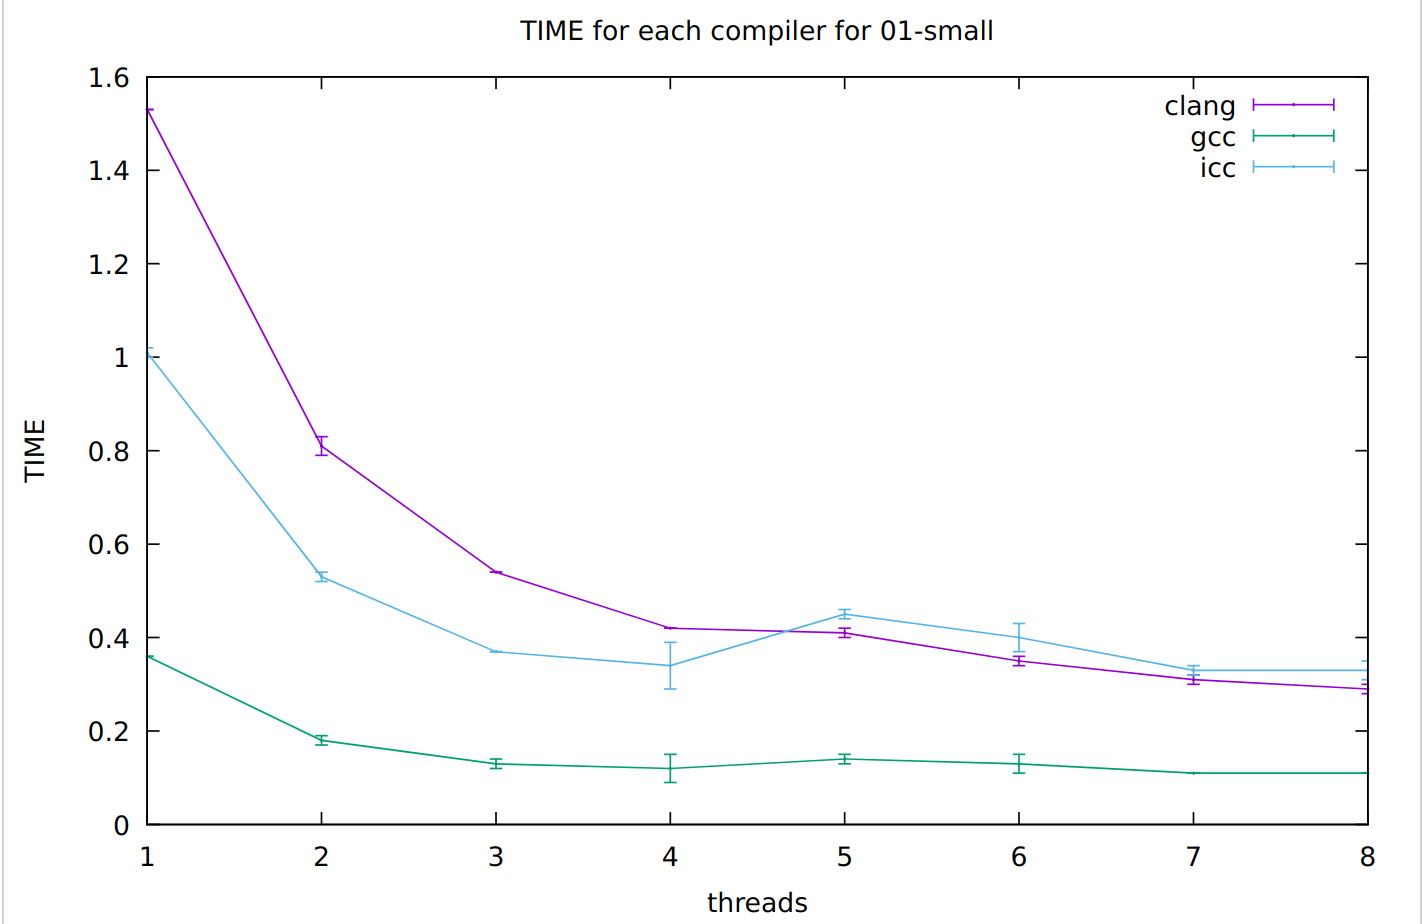
\includegraphics[width=\textwidth]{bucle2=01-small}
    \end{subfigure}
    \caption{\underline{Tamaño pequeño}: Tiempos de ejecución vs nº de hilos}
    \label{fig:bucle2=01-small}
\end{figure}

%%% TABLA DE TIEMPOS E IMÁGENES %%%
\begin{figure}[H]
    \centering
    \begin{subfigure}{0.4\textwidth}
        \begin{adjustbox}{width=\textwidth} 
        \begin{tabular}{|c|c|c|c|c|}
            \hline
            \rowcolor{azul} \multicolumn{2}{|c|}{}&\multicolumn{3}{c|}{\textbf{Compiler}} \\ \hline
            \rowcolor{azul} \multicolumn{2}{|c|}{}&\texttt{clang}&\texttt{gcc}&\texttt{icc}\\ \hline
            \rowcolor{azul} \textbf{Testing size} & \textbf{Threads}&\multicolumn{3}{c|}{\textbf{Average time (s)}} \\ \hline
            \multirow{8}{2.5cm}{\textbf{02-medium}} & 1 & \(4.45\pm{0.03}\) & \(0.89\pm{0.03}\) & \(2.90\pm{0.03}\) \\ \cline{2-5}
            & 2 & \(2.31\pm{0.05}\) & \(0.47\pm{0.02}\) & \(3.37\pm{0.06}\) \\ \cline{2-5}
            & 3 & \(1.52\pm{0.00}\) & \(0.33\pm{0.02}\) & \(2.93\pm{0.05}\) \\ \cline{2-5}
            & 4 & \(1.20\pm{0.03}\) & \(0.30\pm{0.06}\) & \(2.97\pm{0.03}\) \\ \cline{2-5}
            & 5 & \(1.16\pm{0.04}\) & \(0.37\pm{0.02}\) & \(2.96\pm{0.02}\) \\ \cline{2-5}
            & 6 & \(0.97\pm{0.03}\) & \(0.31\pm{0.01}\) & \(2.96\pm{0.07}\) \\ \cline{2-5}
            & 7 & \(0.87\pm{0.05}\) & \(0.27\pm{0.01}\) & \(2.93\pm{0.02}\) \\ \cline{2-5}
            & 8 & \(0.77\pm{0.03}\) & \(0.25\pm{0.01}\) & \(2.92\pm{0.01}\) \\ \hline
        \end{tabular}
        \end{adjustbox}
    \end{subfigure}
    \hfill
    \begin{subfigure}{0.5\textwidth}
        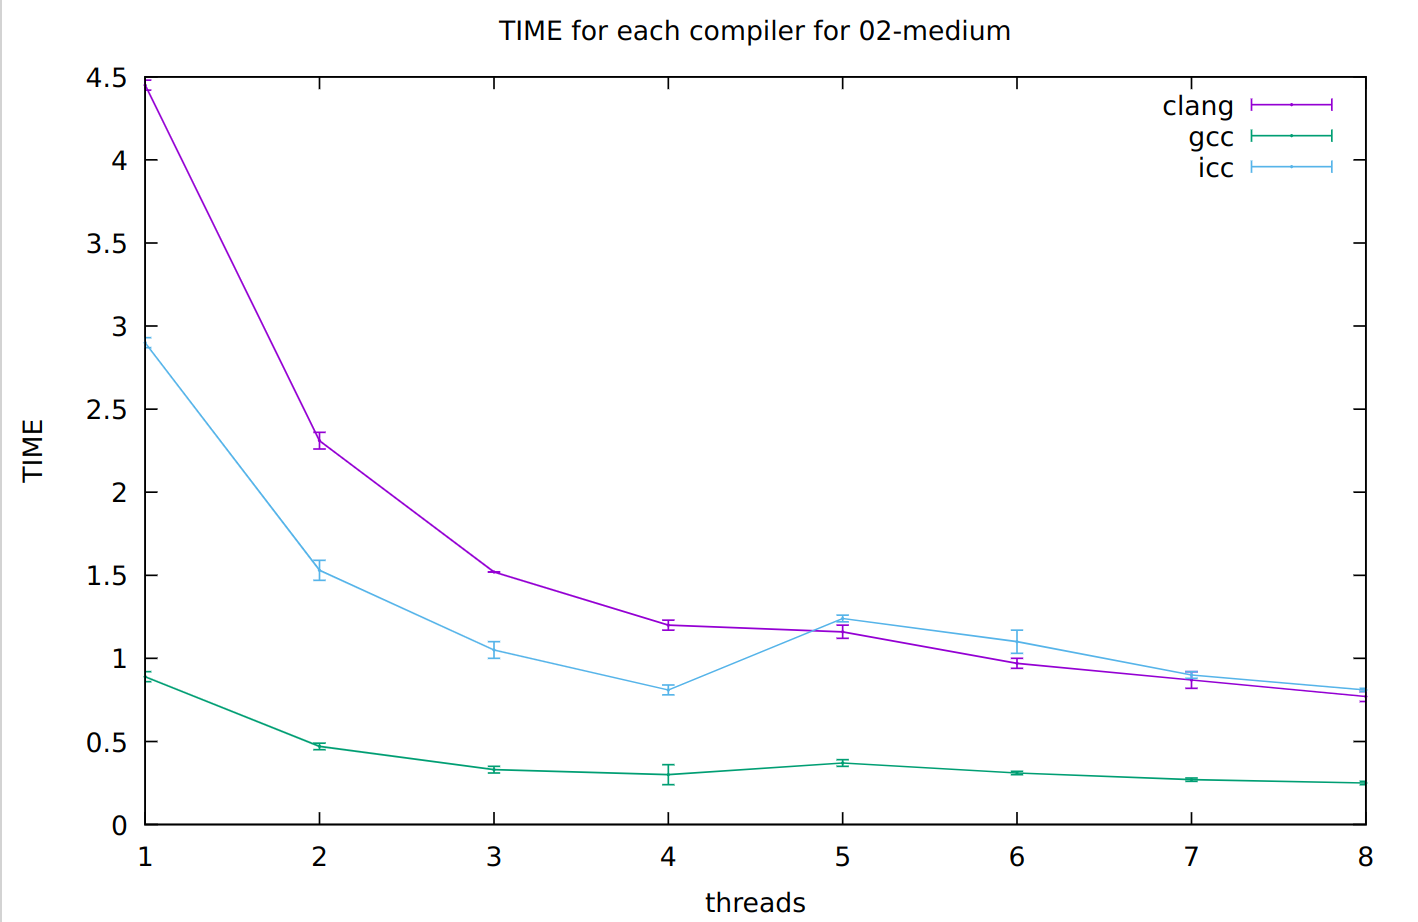
\includegraphics[width=\textwidth]{bucle2=02-medium}
    \end{subfigure}
    \caption{\underline{Tamaño mediano}: Tiempos de ejecución vs nº de hilos}
    \label{bucle2=02-medium}
\end{figure}

%%% TABLA DE TIEMPOS E IMÁGENES %%%
\begin{figure}[H]
    \centering
    \begin{subfigure}{0.4\textwidth}
        \begin{adjustbox}{width=\textwidth} 
        \begin{tabular}{|c|c|c|c|c|}
            \hline
            \rowcolor{azul} \multicolumn{2}{|c|}{}&\multicolumn{3}{c|}{\textbf{Compiler}} \\ \hline
            \rowcolor{azul} \multicolumn{2}{|c|}{}&\texttt{clang}&\texttt{gcc}&\texttt{icc}\\ \hline
            \rowcolor{azul} \textbf{Testing size} & \textbf{Threads}&\multicolumn{3}{c|}{\textbf{Average time (s)}} \\ \hline
            \multirow{8}{1cm}{\textbf{03-large}} & 1 & \(7.62\pm{0.15}\) & \(1.56\pm{0.07}\) & \(5.00\pm{0.12}\) \\ \cline{2-5}
            & 2 & \(3.93\pm{0.05}\) & \(0.80\pm{0.04}\) & \(2.63\pm{0.11}\) \\ \cline{2-5}
            & 3 & \(2.65\pm{0.02}\) & \(0.55\pm{0.04}\) & \(1.85\pm{0.15}\) \\ \cline{2-5}
            & 4 & \(2.02\pm{0.02}\) & \(0.42\pm{0.02}\) & \(1.37\pm{0.05}\) \\ \cline{2-5}
            & 5 & \(1.97\pm{0.12}\) & \(0.60\pm{0.03}\) & \(2.10\pm{0.02}\) \\ \cline{2-5}
            & 6 & \(1.67\pm{0.09}\) & \(0.51\pm{0.02}\) & \(1.78\pm{0.05}\) \\ \cline{2-5}
            & 7 & \(1.43\pm{0.07}\) & \(0.47\pm{0.04}\) & \(1.51\pm{0.02}\) \\ \cline{2-5}
            & 8 & \(1.28\pm{0.06}\) & \(0.41\pm{0.02}\) & \(1.40\pm{0.05}\) \\ \hline
        \end{tabular}
        \end{adjustbox}
    \end{subfigure}
    \hfill
    \begin{subfigure}{0.5\textwidth}
        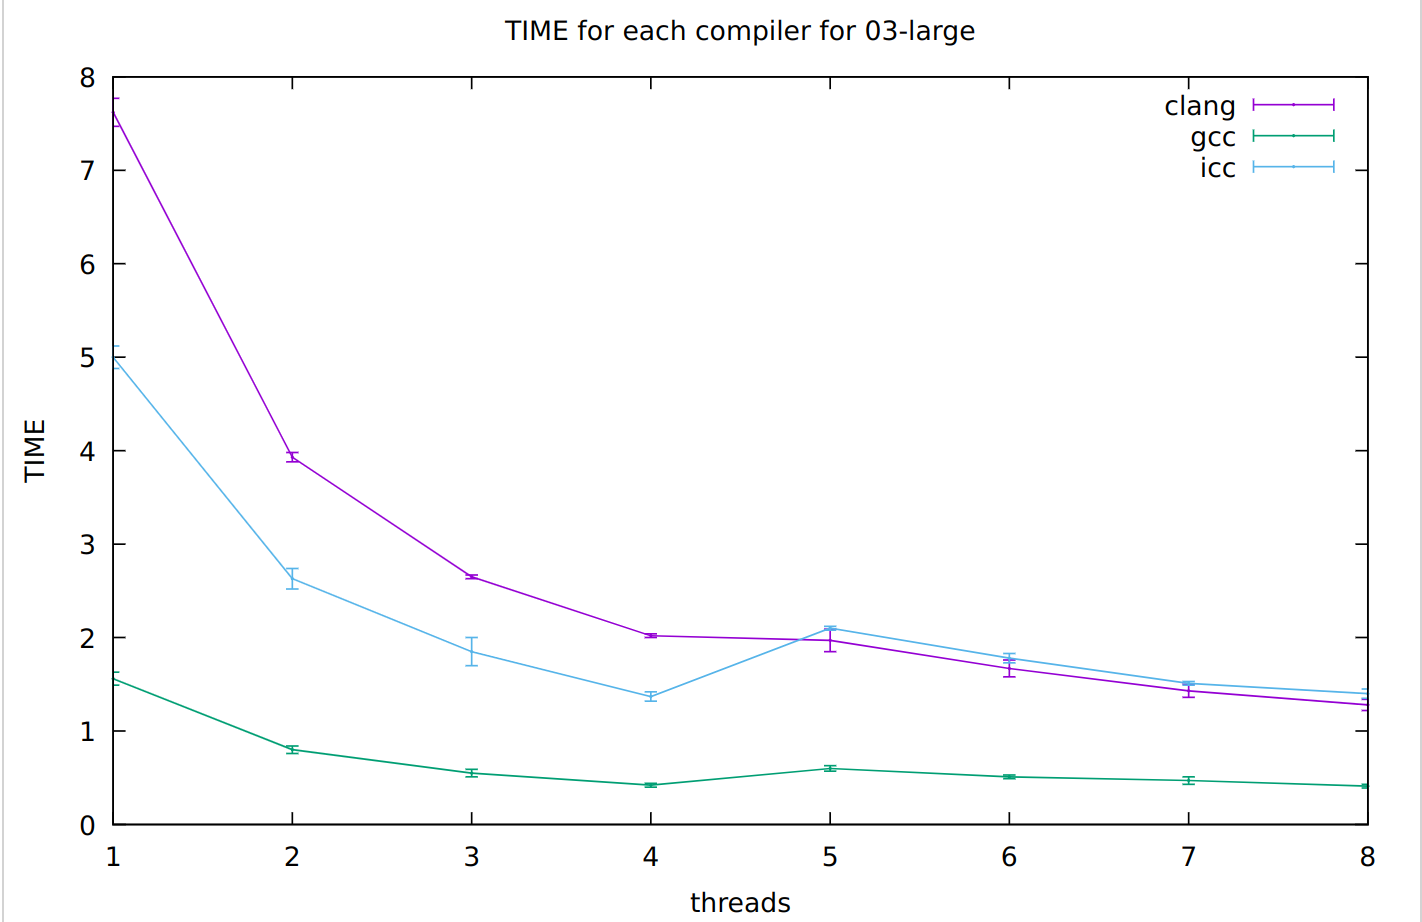
\includegraphics[width=\textwidth]{bucle2=03-large}
    \end{subfigure}
    \caption{\underline{Tamaño largo}: Tiempos de ejecución vs nº de hilos}
    \label{bucle2=03-large}
\end{figure}
\subsubsection{\textbf{4ºBucle:}}
\begin{listing}[firstnumber=31]
    @@ -32,3 +32,3 @@
    for (int i = 0; i < arrays_size; ++i) {
      C[i] = A[i] + 2 * B[i];
    }
\end{listing}
\par No hace falta analizar la ejecución desarrollada del bucle porque mirando el código se puede decir a simple vista que no hay
\textbf{ninguna dependencia} entre iteraciones, porque en cada iteración solo se necesita los valores que se leen y procesan en ella misma.
El compilador podrá vectorizar automáticamente este bucle sin ninguna modificación.
\subsubsection{\textbf{5ºBucle:}}
\begin{listing}[firstnumber=126]
    @@ -127,3 +127,3 @@
    LOOP BEGIN at loops.cpp(36,5)
        remark #15300: LOOP WAS VECTORIZED
    LOOP END
\end{listing}
\par Para saber como optimiza este bucle podemos ver el código ensamblador generado con el comando \texttt{\$ objdump -S loops | less}
en el que se puede ver como utiliza 8 registros para almacenar los totales parciales de ocho en ocho en cada iteración.

\begin{listing}[numbers=none, basicstyle=\scriptsize\ttfamily]
    400ee5: 0f ae f0                mfence
    400ee8: c5 7d 6f d1             vmovdqa %ymm1,%ymm10
    400eec: 33 c0                   xor %eax,%eax
    400eee: c4 41 25 57 db          vxorpd %ymm11,%ymm11,%ymm11
    400ef3: c5 7d 6f c9             vmovdqa %ymm1,%ymm9
    400ef7: c5 7d 6f c1             vmovdqa %ymm1,%ymm8
    400efb: c5 fd 6f f9             vmovdqa %ymm1,%ymm7
    400eff: c5 fd 6f f1             vmovdqa %ymm1,%ymm6
    400f03: c5 fd 28 e9             vmovapd %ymm1,%ymm5
    400f07: c5 fd 28 e1             vmovapd %ymm1,%ymm4
    400f0b: 0f 1f 44 00 00          nopl 0x0(%rax,%rax,1)
    400f10: c5 25 58 1c c5 60 61    vaddpd 0x1546160(,%rax,8),%ymm11,%ymm11
    400f17: 54 01
    400f19: c5 2d 58 14 c5 80 61    vaddpd 0x1546180(,%rax,8),%ymm10,%ymm10
    400f20: 54 01
    400f22: c5 35 58 0c c5 a0 61    vaddpd 0x15461a0(,%rax,8),%ymm9,%ymm9
    400f29: 54 01
    400f2b: c5 3d 58 04 c5 c0 61    vaddpd 0x15461c0(,%rax,8),%ymm8,%ymm8
    400f32: 54 01
    400f34: c5 c5 58 3c c5 e0 61    vaddpd 0x15461e0(,%rax,8),%ymm7,%ymm7
    400f3b: 54 01
    400f3d: c5 cd 58 34 c5 00 62    vaddpd 0x1546200(,%rax,8),%ymm6,%ymm6
    400f44: 54 01
    400f46: c5 d5 58 2c c5 20 62    vaddpd 0x1546220(,%rax,8),%ymm5,%ymm5
    400f4d: 54 01
    400f4f: c5 dd 58 24 c5 40 62    vaddpd 0x1546240(,%rax,8),%ymm4,%ymm4
    400f56: 54 01
    400f58: 48 83 c0 20             add $0x20,%rax
    400f5c: 48 3d 40 42 0f 00       cmp $0xf4240,%rax
    400f62: 72 ac                   jb 400f10 <main+0x200>
    400f64: c4 41 25 58 d2          vaddpd %ymm10,%ymm11,%ymm10
    400f69: fe c1                   inc %cl
    400f6b: c4 41 35 58 c0          vaddpd %ymm8,%ymm9,%ymm8
    400f70: c5 c5 58 f6             vaddpd %ymm6,%ymm7,%ymm6
    400f74: c5 d5 58 e4             vaddpd %ymm4,%ymm5,%ymm4
    400f78: c4 41 2d 58 c8          vaddpd %ymm8,%ymm10,%ymm9
    400f7d: c5 cd 58 ec             vaddpd %ymm4,%ymm6,%ymm5
    400f81: c5 b5 58 fd             vaddpd %ymm5,%ymm9,%ymm7
    400f85: c4 c3 7d 19 fb 01       vextractf128 $0x1,%ymm7,%xmm11
    400f8b: c4 41 41 58 e3          vaddpd %xmm11,%xmm7,%xmm12
    400f90: c4 41 19 15 ec          vunpckhpd %xmm12,%xmm12,%xmm13
    400f95: c4 41 1b 58 f5          vaddsd %xmm13,%xmm12,%xmm14
    400f9a: c5 8b 58 c0             vaddsd %xmm0,%xmm14,%xmm0
    400f9e: 80 f9 64                cmp $0x64,%cl
    400fa1: 0f 82 b2 fd ff ff       jb 400d59 <main+0x49>
\end{listing}
\par En \texttt{C} el código equivalente sería:
\begin{listing}[firstnumber=35]
    @@ -36,3 +36,11 @@
    + for (int i = 0; i < arrays_size; i+=8)
    + {
    +    ymm11 = ymm11 + c[i];
    +    ymm10 = ymm10 + c[i+1];
    +    ymm9 = ymm9 + c[i+2];
    +    ymm8 = ymm8 + c[i+3];
    +    ymm7 = ymm7 + c[i+4];
    +    ymm6 = ymm6 + c[i+5];
    +    ymm5 = ymm5 + c[i+6];
    +    ymm4 = ymm4 + c[i+7];
    + }
    + total = ymm11+ymm10+ymm9+ymm8+ymm7+ymm6+ymm5+ymm4+total;
\end{listing}
\subsection{Transformación manual para vectorizar}


\subsubsection{\textbf{1ºBucle:}}
\par El primer bucle es \texttt{while(difference / (state.height * state.width) > tolerance)}. Se podría paralelizar creando una rama master y añadiendo un pragma de tipo
\texttt{task} que comparte la variable \texttt{iterations} antes del \texttt{if(verbose)} porque la ejecución de la siguiente iteración no depende de esto.
Además, dentro de esta \texttt{task} se necesita un pragma \texttt{atomic}, porque solo un hilo puede modificar a la vez esa variable global. Esta
implementación, mostrada en el código siguiente, no ayuda mucho en el rendimiento de la aplicación y la mejora es despreciable e incluso en 
algunos casos es peor como se indica en todas las tablas y gráficas.
%%% TABLA DE TIEMPOS E IMÁGENES %%%
\begin{figure}[H]
    \centering
    \begin{subfigure}{0.4\textwidth}
        \begin{adjustbox}{width=\textwidth} 
        \begin{tabular}{|c|c|c|c|c|}
            \hline
            \rowcolor{azul} \multicolumn{2}{|c|}{}&\multicolumn{3}{c|}{\textbf{Compiler}} \\ \hline
            \rowcolor{azul} \multicolumn{2}{|c|}{}&\texttt{clang}&\texttt{gcc}&\texttt{icc}\\ \hline
            \rowcolor{azul} \textbf{Testing size} & \textbf{Threads}&\multicolumn{3}{c|}{\textbf{Average time (s)}} \\ \hline
            \multirow{8}{1cm}{\textbf{01-small}} & 1 & \(1.58\pm{0.03}\) & \(0.32\pm{0.01}\) & \(1.00\pm{0.01}\) \\ \cline{2-5}
            & 2 & \(1.58\pm{0.03}\) & \(0.32\pm{0.01}\) & \(1.02\pm{0.01}\) \\ \cline{2-5}
            & 3 & \(1.60\pm{0.03}\) & \(0.33\pm{0.01}\) & \(1.02\pm{0.01}\) \\ \cline{2-5}
            & 4 & \(1.62\pm{0.01}\) & \(0.33\pm{0.01}\) & \(1.08\pm{0.04}\) \\ \cline{2-5}
            & 5 & \(1.62\pm{0.01}\) & \(0.33\pm{0.01}\) & \(1.05\pm{0.01}\) \\ \cline{2-5}
            & 6 & \(1.72\pm{0.01}\) & \(0.46\pm{0.01}\) & \(1.41\pm{0.35}\) \\ \cline{2-5}
            & 7 & \(1.99\pm{0.01}\) & \(0.47\pm{0.01}\) & \(1.44\pm{0.32}\) \\ \cline{2-5}
            & 8 & \(1.85\pm{0.01}\) & \(0.47\pm{0.02}\) & \(1.77\pm{0.02}\) \\ \hline
        \end{tabular}
        \end{adjustbox}
    \end{subfigure}
    \hfill
    \begin{subfigure}{0.5\textwidth}
        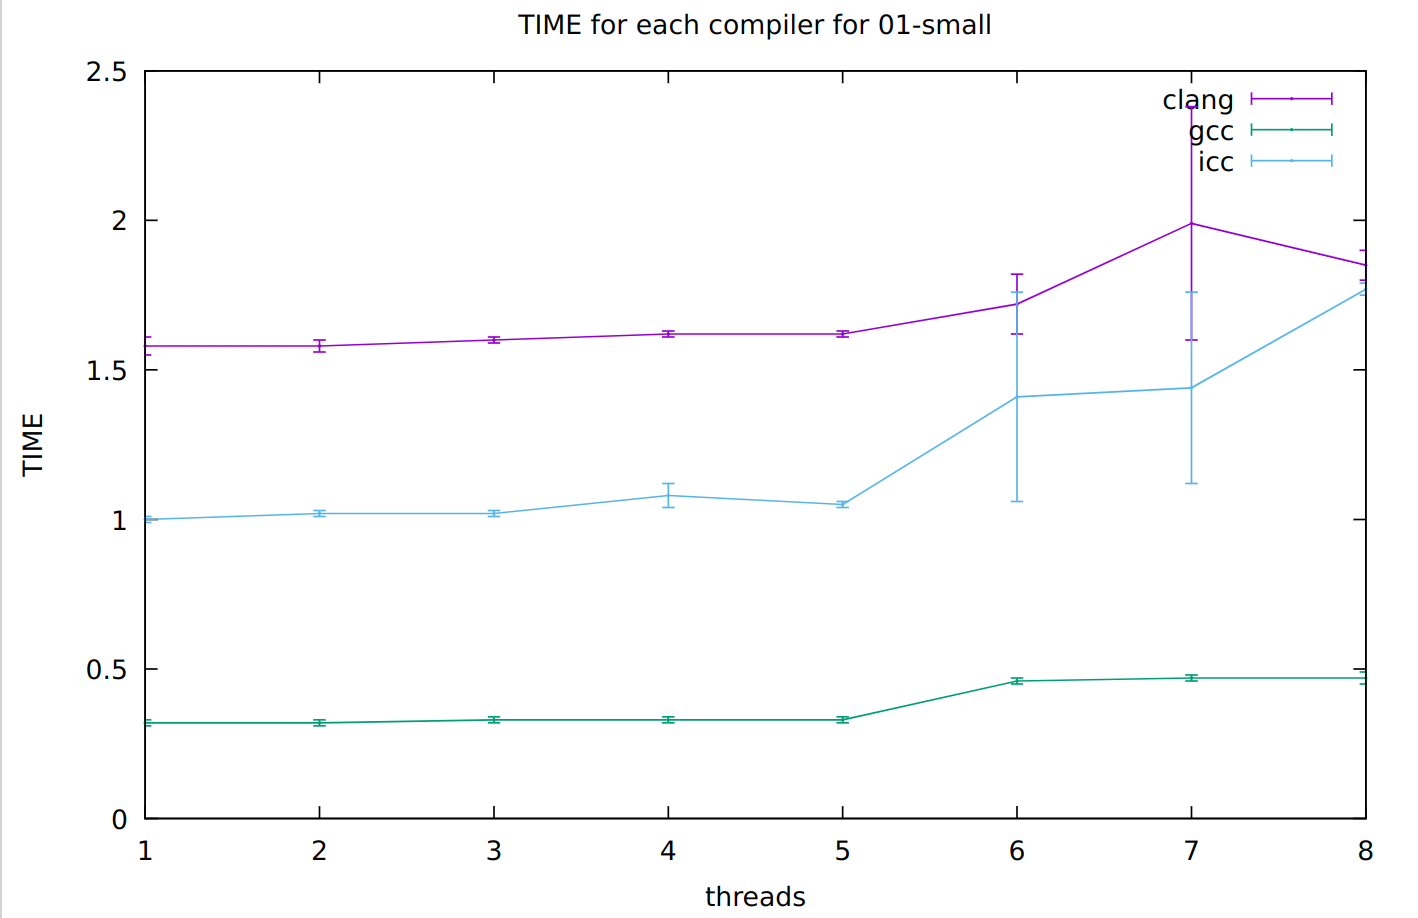
\includegraphics[width=\textwidth]{bucle1=01-small}
    \end{subfigure}
    \caption{\underline{1º Bucle, tamaño pequeño}: Tiempos de ejecución vs nº de hilos}
    \label{fig:bucle1=01-small}
\end{figure}
\newpage

\subsubsection{\textbf{heat.cpp}}
\begin{listing}[firstnumber=20]
    @@ -21,28 +21,36 @@
    void solve(Matrix<double>& state, double tolerance, int& iterations, double& last_difference) {
    Matrix<double> next_state = state;
    iterations = 0;
    double difference;
  + #pragma omp parallel
  + {
  + #pragma omp master
    do {
        difference = 0;
        for (size_t i = 1; i < state.height - 1; ++i) {
            for (size_t j = 1; j < state.width - 1; ++j) {
                next_state[i][j] = (state[i][j]
                                + state[i + 1][j]  
                                + state[i - 1][j]  
                                + state[i][j + 1]  
                                + state[i][j - 1]) / 5;
                difference = difference 
                             + abs(next_state[i][j]-state[i][j]);
            }
        }

        state.swap_data(next_state);

  + #pragma omp task shared(iterations)
  + {    
        if (verbose) {
            cout << "Iteration " << iterations << ":" << endl;
            printf_matrix("%7.3f", state);
            cout << "Difference: " << difference << endl;
        }
  + #pragma omp atomic
        ++iterations;
  + }
    } while (difference / (state.height * state.width) > tolerance);
    last_difference = difference / (state.height * state.width);
  + }
    }
\end{listing}


%%% TABLA DE TIEMPOS E IMÁGENES %%%
\begin{figure}[H]
    \centering
    \begin{subfigure}{0.4\textwidth}
        \begin{adjustbox}{width=\textwidth} 
        \begin{tabular}{|c|c|c|c|c|}
            \hline
            \rowcolor{azul} \multicolumn{2}{|c|}{}&\multicolumn{3}{c|}{\textbf{Compiler}} \\ \hline
            \rowcolor{azul} \multicolumn{2}{|c|}{}&\texttt{clang}&\texttt{gcc}&\texttt{icc}\\ \hline
            \rowcolor{azul} \textbf{Testing size} & \textbf{Threads}&\multicolumn{3}{c|}{\textbf{Average time (s)}} \\ \hline
            \multirow{8}{2.5cm}{\textbf{02-medium}} & 1 & \(4.83\pm{0.42}\) & \(0.89\pm{0.04}\) & \(2.88\pm{0.04}\) \\ \cline{2-5}
            & 2 & \(4.73\pm{0.24}\) & \(0.91\pm{0.04}\) & \(2.94\pm{0.04}\) \\ \cline{2-5}
            & 3 & \(4.57\pm{0.07}\) & \(0.90\pm{0.03}\) & \(3.22\pm{0.22}\) \\ \cline{2-5}
            & 4 & \(5.19\pm{0.57}\) & \(0.93\pm{0.04}\) & \(3.19\pm{0.21}\) \\ \cline{2-5}
            & 5 & \(4.63\pm{0.04}\) & \(1.28\pm{0.03}\) & \(3.16\pm{0.15}\) \\ \cline{2-5}
            & 6 & \(4.63\pm{0.03}\) & \(1.27\pm{0.03}\) & \(4.20\pm{0.86}\) \\ \cline{2-5}
            & 7 & \(4.64\pm{0.03}\) & \(1.27\pm{0.03}\) & \(4.83\pm{0.24}\) \\ \cline{2-5}
            & 8 & \(5.41\pm{0.08}\) & \(1.20\pm{0.04}\) & \(5.17\pm{0.10}\) \\ \hline
        \end{tabular}
        \end{adjustbox}
    \end{subfigure}
    \hfill
    \begin{subfigure}{0.5\textwidth}
        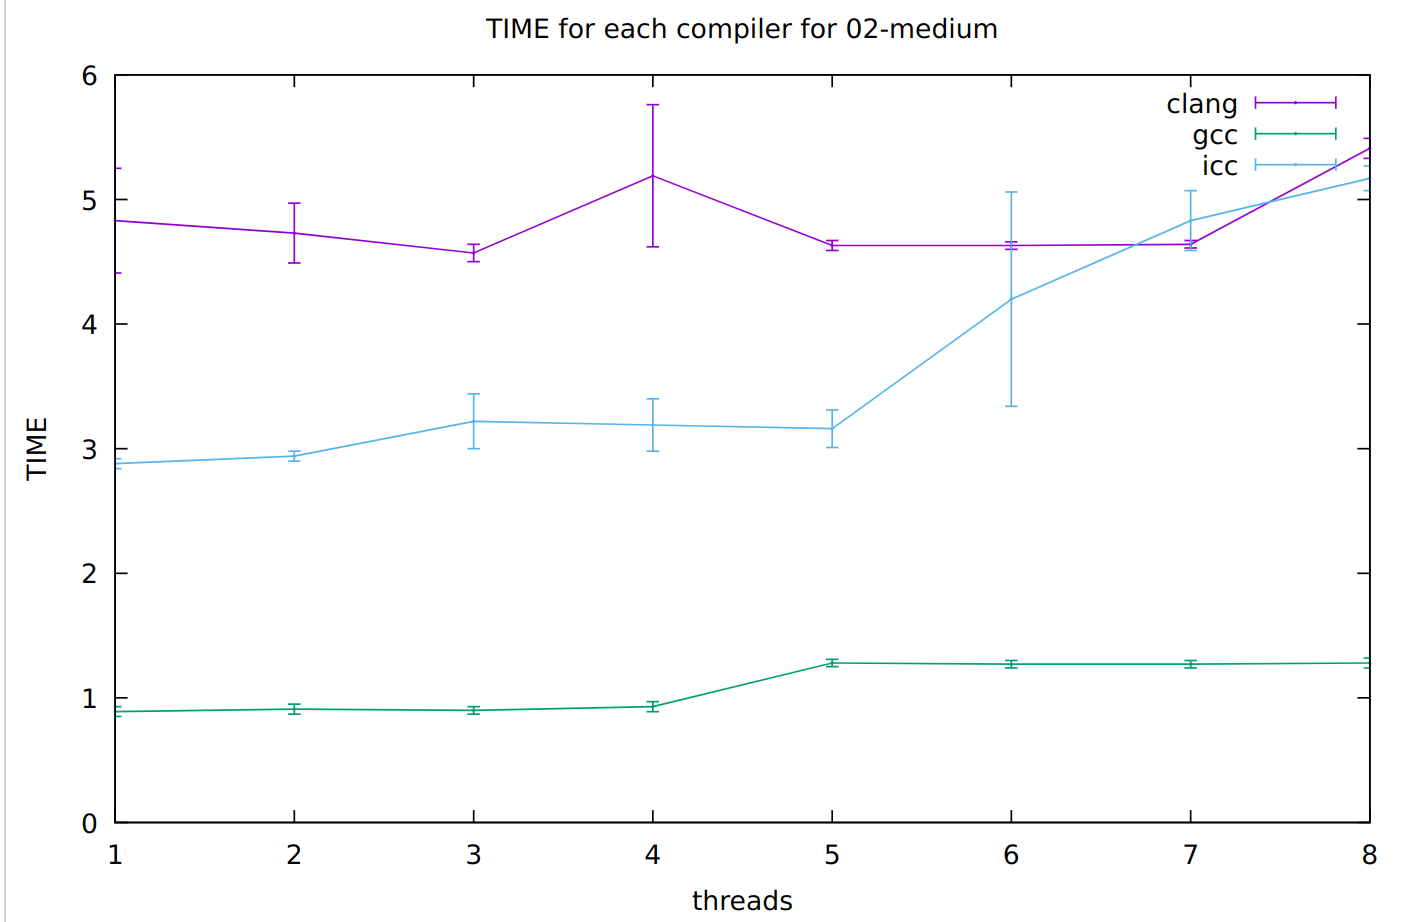
\includegraphics[width=\textwidth]{bucle1=02-medium}
    \end{subfigure}
    \caption{\underline{1º Bucle, tamaño mediano}: Tiempos de ejecución vs nº de hilos}
    \label{bucle1=02-medium}
\end{figure}

%%% TABLA DE TIEMPOS E IMÁGENES %%%
\begin{figure}[H]
    \centering
    \begin{subfigure}{0.4\textwidth}
        \begin{adjustbox}{width=\textwidth} 
        \begin{tabular}{|c|c|c|c|c|}
            \hline
            \rowcolor{azul} \multicolumn{2}{|c|}{}&\multicolumn{3}{c|}{\textbf{Compiler}} \\ \hline
            \rowcolor{azul} \multicolumn{2}{|c|}{}&\texttt{clang}&\texttt{gcc}&\texttt{icc}\\ \hline
            \rowcolor{azul} \textbf{Testing size} & \textbf{Threads}&\multicolumn{3}{c|}{\textbf{Average time (s)}} \\ \hline
            \multirow{8}{1cm}{\textbf{03-large}} & 1 & \(7.58\pm{0.01}\) & \(1.54\pm{0.11}\) & \(4.97\pm{0.13}\) \\ \cline{2-5}
            & 2 & \(7.69\pm{0.05}\) & \(1.55\pm{0.07}\) & \(5.11\pm{0.16}\) \\ \cline{2-5}
            & 3 & \(7.83\pm{0.01}\) & \(1.56\pm{0.08}\) & \(5.20\pm{0.21}\) \\ \cline{2-5}
            & 4 & \(7.87\pm{0.06}\) & \(1.61\pm{0.09}\) & \(5.23\pm{0.16}\) \\ \cline{2-5}
            & 5 & \(7.90\pm{0.03}\) & \(2.19\pm{0.05}\) & \(5.23\pm{0.18}\) \\ \cline{2-5}
            & 6 & \(7.87\pm{0.05}\) & \(2.17\pm{0.05}\) & \(5.20\pm{0.14}\) \\ \cline{2-5}
            & 7 & \(8.86\pm{0.01}\) & \(2.16\pm{0.06}\) & \(8.78\pm{0.18}\) \\ \cline{2-5}
            & 8 & \(8.85\pm{0.03}\) & \(2.15\pm{0.03}\) & \(8.76\pm{0.15}\) \\ \hline
        \end{tabular}
        \end{adjustbox}
    \end{subfigure}
    \hfill
    \begin{subfigure}{0.5\textwidth}
        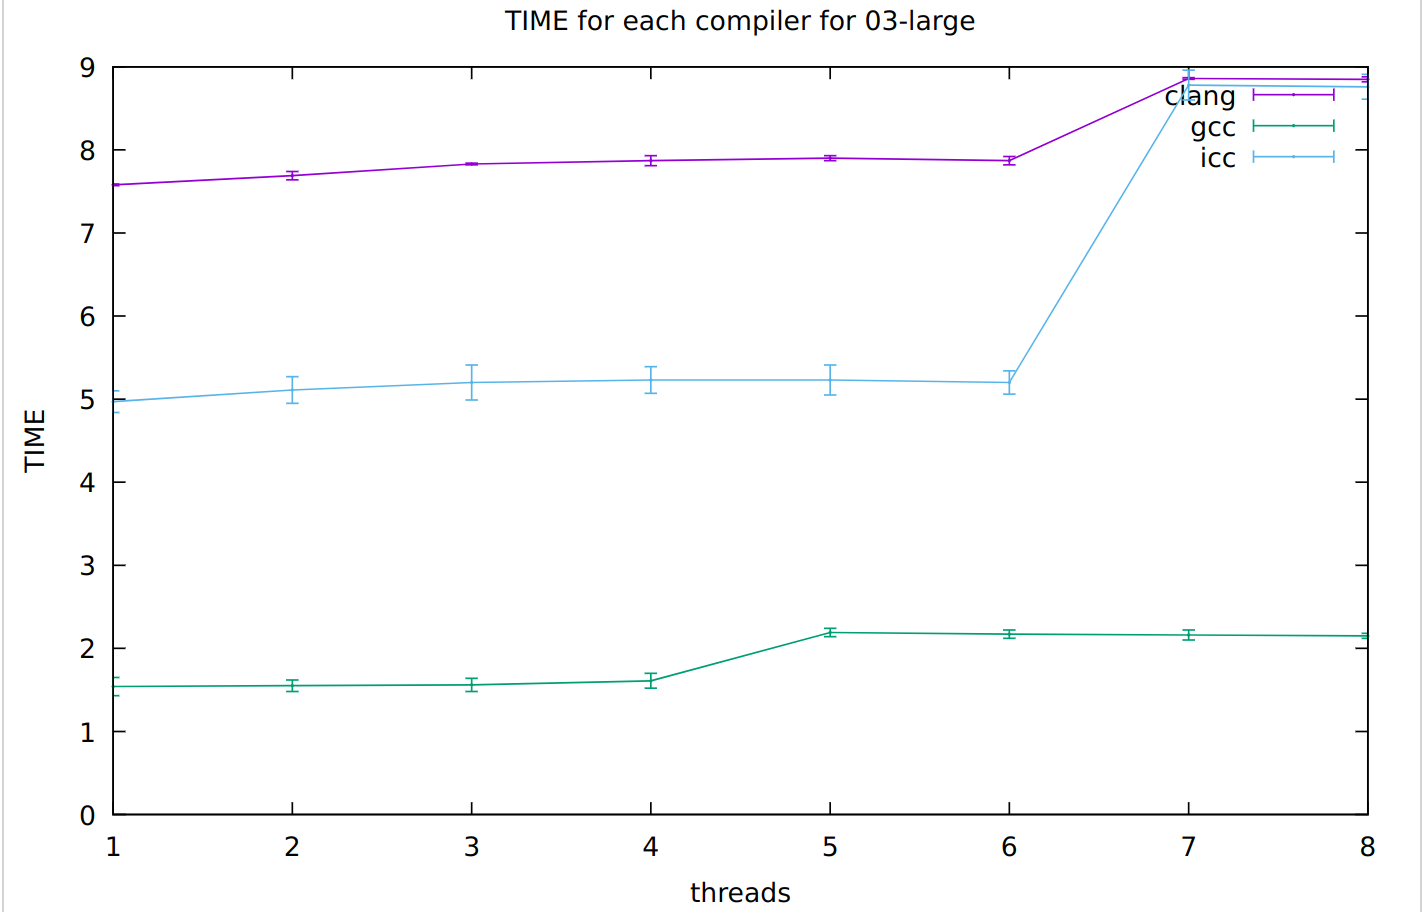
\includegraphics[width=\textwidth]{bucle1=03-large}
    \end{subfigure}
    \caption{\underline{1º Bucle, tamaño largo}: Tiempos de ejecución vs nº de hilos}
    \label{bucle1=03-large}
\end{figure}
\subsubsection{\textbf{3ºBucle:}}
\begin{listing}
    @@ -20,3 +20,4 @@
\end{listing}

\par El primer y tercer bucle no se pueden vectorizar de forma automática porque tiene dependencias. No son inmediatamente
vectorizables, tampoco se puede reorganizar el código para evitar las dependencias ni crear instrucciones parciales para mitigar la
dependencia. No he encontrado ninguna transformación manual para poder vectorizarlos. Separar cada bucle en dos sería
ineficiente y el compilador descarta la vectorización de la instrucción que ya no tendría dependencia por tanto este cambio no
sería una solución. A lo mejor se puede programar usando los instrinsics vectoriales, que son un conjunto de funciones
disponibles para lenguajes de alto nivel que corresponden directamente a instrucciones vectoriales o hay alguna librería
optimizada que ya esté vectorizada porque la idea de programar en lenguaje ensamblador hoy en día casi nunca se realiza.
%%%%%%%%%%%%%%%%%%%%%% Procesadores CMP: usando la vectorización y la paralelización - EJERCICIO 2 %%%%%%%%%%%%%%%%%%%%%%
\newpage
\section{Ejercicio 2}
\subsection{Enunciado}
\begin{ejer}
    \textbf{2.-} En el directorio \texttt{paralelización} hay un pequeño programa que simula la propagación del 
    calor en una superficie rectangular. Se supone que la temperatura de cada uno de los bordes de la
    superficie se mantiene constante y el programa calcula la temperatura final de cada punto de
    la superficie representada como una matriz. Para ello utiliza un algoritmo iterativo tipo \texttt{stencil},
    el cual actualiza cada uno de los elementos de la matriz en función del valor previo del mismo
    elemento y sus vecinos.
    \par El código principal del algoritmo se encuentra en el fichero \texttt{heat.cpp}, que será el único que se
    necesitará modificar. Además, el fichero \texttt{matrix.h} proporciona un tipo de datos para almacenar las
    matrices utilizadas por el algoritmo, mientras que el fichero \texttt{main.cpp} incluye el código necesario
    para ejecutar el programa y medir el tiempo empleado en realizar la simulación. El programa permite
     configurar múltiples parámetros de la ejecución mediante opciones de la línea de comandos 
     (ver \texttt{main.cpp}).
    \par Además del programa, se incluye un \texttt{Makefile} para compilarlo usando tanto el compilador \texttt{GCC}
    como el \texttt{ICC}. Se incluyen también scripts para automatizar la comprobación de que los resultados
    son correctos y para automatizar la medida del tiempo de ejecución del programa usando diferente
    número de hilos (generando ficheros \texttt{tsv} que se pueden utilizar para generar gráficas fácilmente
    con multitud de programas, incluyendo cualquier hoja de cálculo). Se aconseja el uso de un
    ordenador que tenga 4 cores o más. Finalmente, se incluyen tres casos de prueba y su salida
    correspondiente, que se utilizarán para comprobar la corrección del programa modificado y para
    medir su rendimiento. El \texttt{Makefile} incluye objetivos para ejecutar todos los tests
    (\texttt{make tests} o \texttt{make tests-icc}) y para realizar la toma de tiempos (\texttt{make times} o
     \texttt{make times-icc}).
    \par Para completar este ejercicio, realiza lo siguiente:
    \begin{itemize}
        \item El procedimiento \texttt{solve} de \texttt{heat.cpp} tiene 3 bucles. Identifícalos y explica para cada uno
        de ellos si es candidato para la paralelización usando OpenMP. Indica en cada caso qué
        \texttt{pragma} (o \texttt{pragmas}) sería necesario añadir para realizar la paralelización correctamente.
        Presta especial cuidado a la clasificación de las variables (ya sean de reducción, compartidas
        o privadas).
        \item Prueba a paralelizar individualmente cada uno de los bucles paralelizables y prueba también a
        paralelizar todos los bucles paralelizables a la vez. Para cada versión resultante del programa,
        mide el tiempo de ejecución con diferente número de hilos de cada uno de los tres casos de
        prueba incluidos y genera las correspondientes gráficas mostrando el tiempo de ejecución y
        la escalabilidad obtenida (similar a las figuras \ref{fig:p2enun2-1} y \ref{fig:p2enun2-2}). Comenta los resultados.
    \end{itemize}
\end{ejer}
 %%% IMÁGENES %%%
\begin{figure}
    \centering
    \begin{subfigure}{0.4\textwidth}
        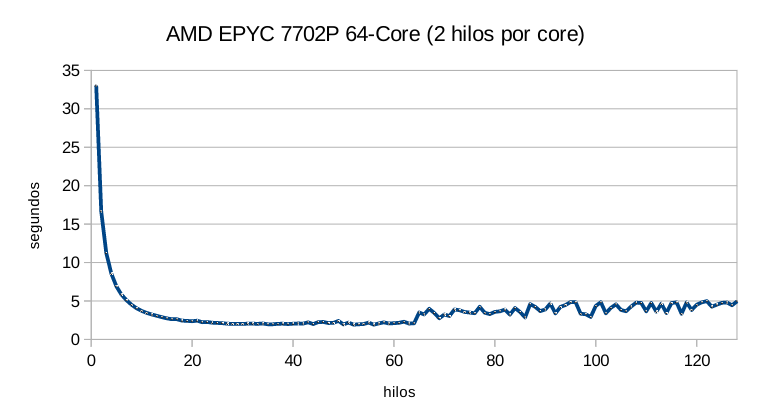
\includegraphics[width=\textwidth]{p2enun2-1}
        \caption{Tiempo de ejecución vs nº de hilos}
        \label{fig:p2enun2-1}
    \end{subfigure}
    \begin{subfigure}{0.4\textwidth}
        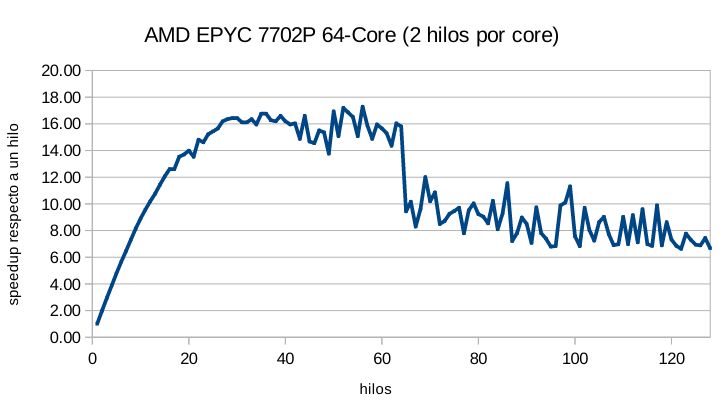
\includegraphics[width=\textwidth]{p2enun2-2}
        \caption{Escalabilidad de la aplicación}
        \label{fig:p2enun2-2}
    \end{subfigure}
\end{figure}

\subsection{Tiempos y gráficas}


\subsubsection{\textbf{Código inicial sin paralelización:}}

\par En estas tres tablas y gráficas (\ref{fig:sin-cambios=01-small}, \ref{sin-cambios=02-medium} y \ref{sin-cambios=03-large}) se muestran los tiempos de ejecución dependiendo del número de hilos,
 tipo de compilador y el tamaño del problema.

\definecolor{azul}{rgb}{0.36, 0.54, 0.66}

%%% TABLA DE TIEMPOS E IMÁGENES %%%
\begin{figure}[H]
    \centering
    \begin{subfigure}{0.4\textwidth}
        \begin{adjustbox}{width=\textwidth} 
        \begin{tabular}{|c|c|c|c|c|}
            \hline
            \rowcolor{azul} \multicolumn{2}{|c|}{}&\multicolumn{3}{c|}{\textbf{Compiler}} \\ \hline
            \rowcolor{azul} \multicolumn{2}{|c|}{}&\texttt{clang}&\texttt{gcc}&\texttt{icc}\\ \hline
            \rowcolor{azul} \textbf{Testing size} & \textbf{Threads}&\multicolumn{3}{c|}{\textbf{Average time (s)}} \\ \hline
            \multirow{8}{1cm}{\textbf{01-small}} & 1 & \(0.83\pm{0.01}\) & \(0.39\pm{0.02}\) & \(1.27\pm{0.06}\) \\ \cline{2-5}
            & 2 & \(0.86\pm{0.03}\) & \(0.34\pm{0.02}\) & \(1.49\pm{0.42}\) \\ \cline{2-5}
            & 3 & \(0.86\pm{0.03}\) & \(0.42\pm{0.05}\) & \(1.02\pm{0.00}\) \\ \cline{2-5}
            & 4 & \(0.84\pm{0.01}\) & \(0.46\pm{0.08}\) & \(1.02\pm{0.00}\) \\ \cline{2-5}
            & 5 & \(0.83\pm{0.01}\) & \(0.45\pm{0.01}\) & \(1.01\pm{0.00}\) \\ \cline{2-5}
            & 6 & \(0.83\pm{0.01}\) & \(0.39\pm{0.02}\) & \(1.01\pm{0.00}\) \\ \cline{2-5}
            & 7 & \(0.83\pm{0.01}\) & \(0.40\pm{0.01}\) & \(1.02\pm{0.00}\) \\ \cline{2-5}
            & 8 & \(0.83\pm{0.01}\) & \(0.40\pm{0.01}\) & \(1.05\pm{0.02}\) \\ \hline
        \end{tabular}
        \end{adjustbox}
    \end{subfigure}
    \hfill
    \begin{subfigure}{0.5\textwidth}
        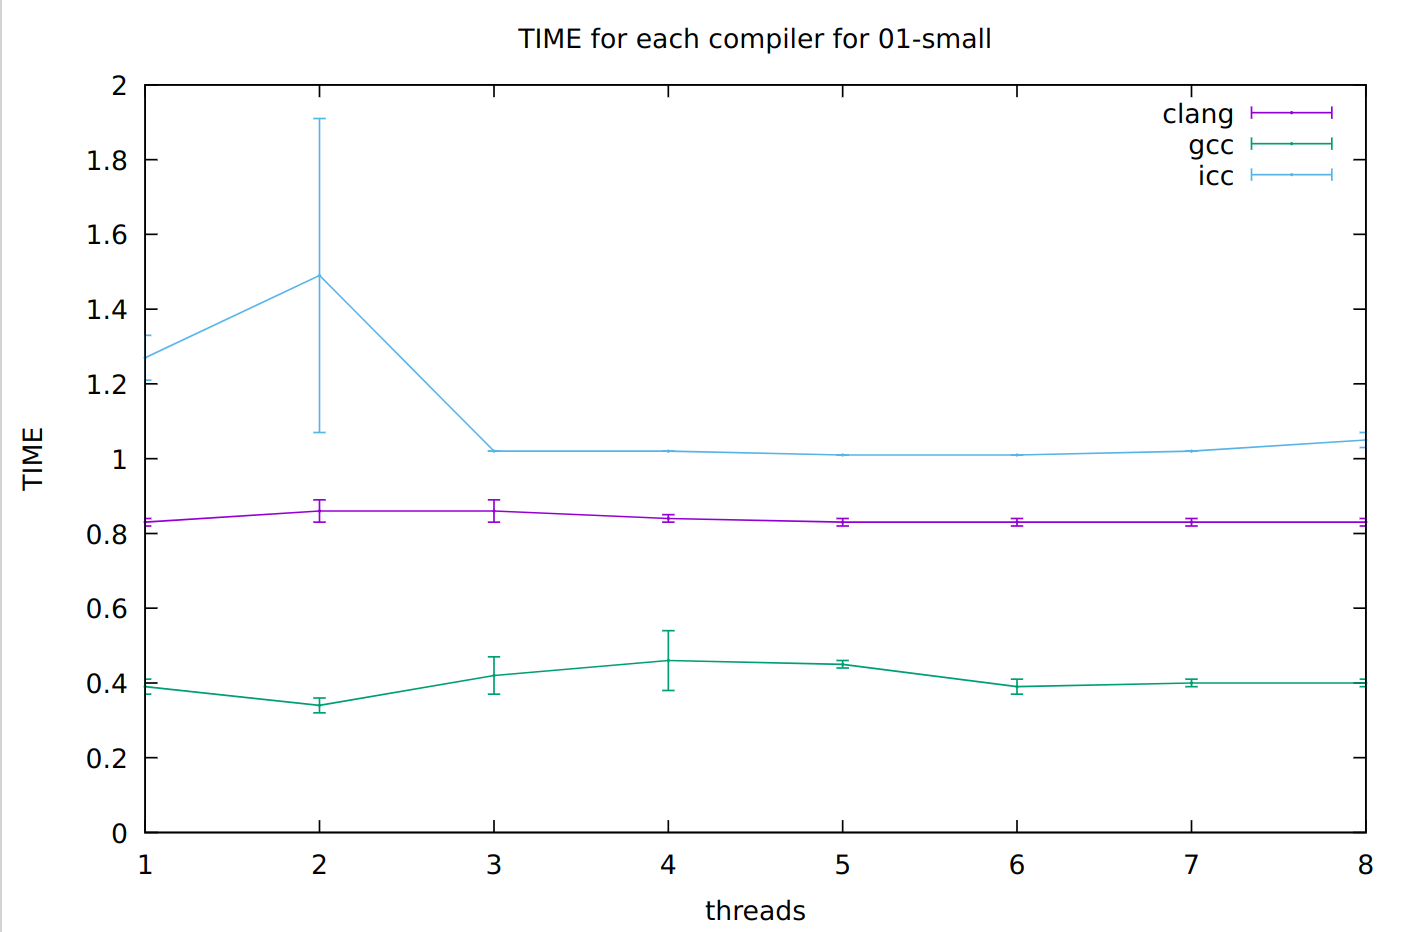
\includegraphics[width=\textwidth]{sin-cambios=01-small}
    \end{subfigure}
    \caption{\underline{Tamaño pequeño}: Tiempos de ejecución vs nº de hilos}
    \label{fig:sin-cambios=01-small}
\end{figure}

%%% TABLA DE TIEMPOS E IMÁGENES %%%
\begin{figure}[H]
    \centering
    \begin{subfigure}{0.4\textwidth}
        \begin{adjustbox}{width=\textwidth} 
        \begin{tabular}{|c|c|c|c|c|}
            \hline
            \rowcolor{azul} \multicolumn{2}{|c|}{}&\multicolumn{3}{c|}{\textbf{Compiler}} \\ \hline
            \rowcolor{azul} \multicolumn{2}{|c|}{}&\texttt{clang}&\texttt{gcc}&\texttt{icc}\\ \hline
            \rowcolor{azul} \textbf{Testing size} & \textbf{Threads}&\multicolumn{3}{c|}{\textbf{Average time (s)}} \\ \hline
            \multirow{8}{2.5cm}{\textbf{02-medium}} & 1 & \(2.38\pm{0.02}\) & \(1.15\pm{0.25}\) & \(2.91\pm{0.07}\) \\ \cline{2-5}
            & 2 & \(2.47\pm{0.10}\) & \(1.18\pm{0.24}\) & \(3.37\pm{0.39}\) \\ \cline{2-5}
            & 3 & \(2.38\pm{0.02}\) & \(1.33\pm{0.44}\) & \(2.93\pm{0.08}\) \\ \cline{2-5}
            & 4 & \(2.41\pm{0.05}\) & \(1.20\pm{0.31}\) & \(2.97\pm{0.12}\) \\ \cline{2-5}
            & 5 & \(2.42\pm{0.05}\) & \(1.20\pm{0.30}\) & \(2.96\pm{0.12}\) \\ \cline{2-5}
            & 6 & \(2.43\pm{0.06}\) & \(1.19\pm{0.29}\) & \(2.96\pm{0.12}\) \\ \cline{2-5}
            & 7 & \(2.38\pm{0.02}\) & \(1.87\pm{0.34}\) & \(2.93\pm{0.07}\) \\ \cline{2-5}
            & 8 & \(2.39\pm{0.03}\) & \(1.40\pm{0.25}\) & \(2.92\pm{0.07}\) \\ \hline
        \end{tabular}
        \end{adjustbox}
    \end{subfigure}
    \hfill
    \begin{subfigure}{0.5\textwidth}
        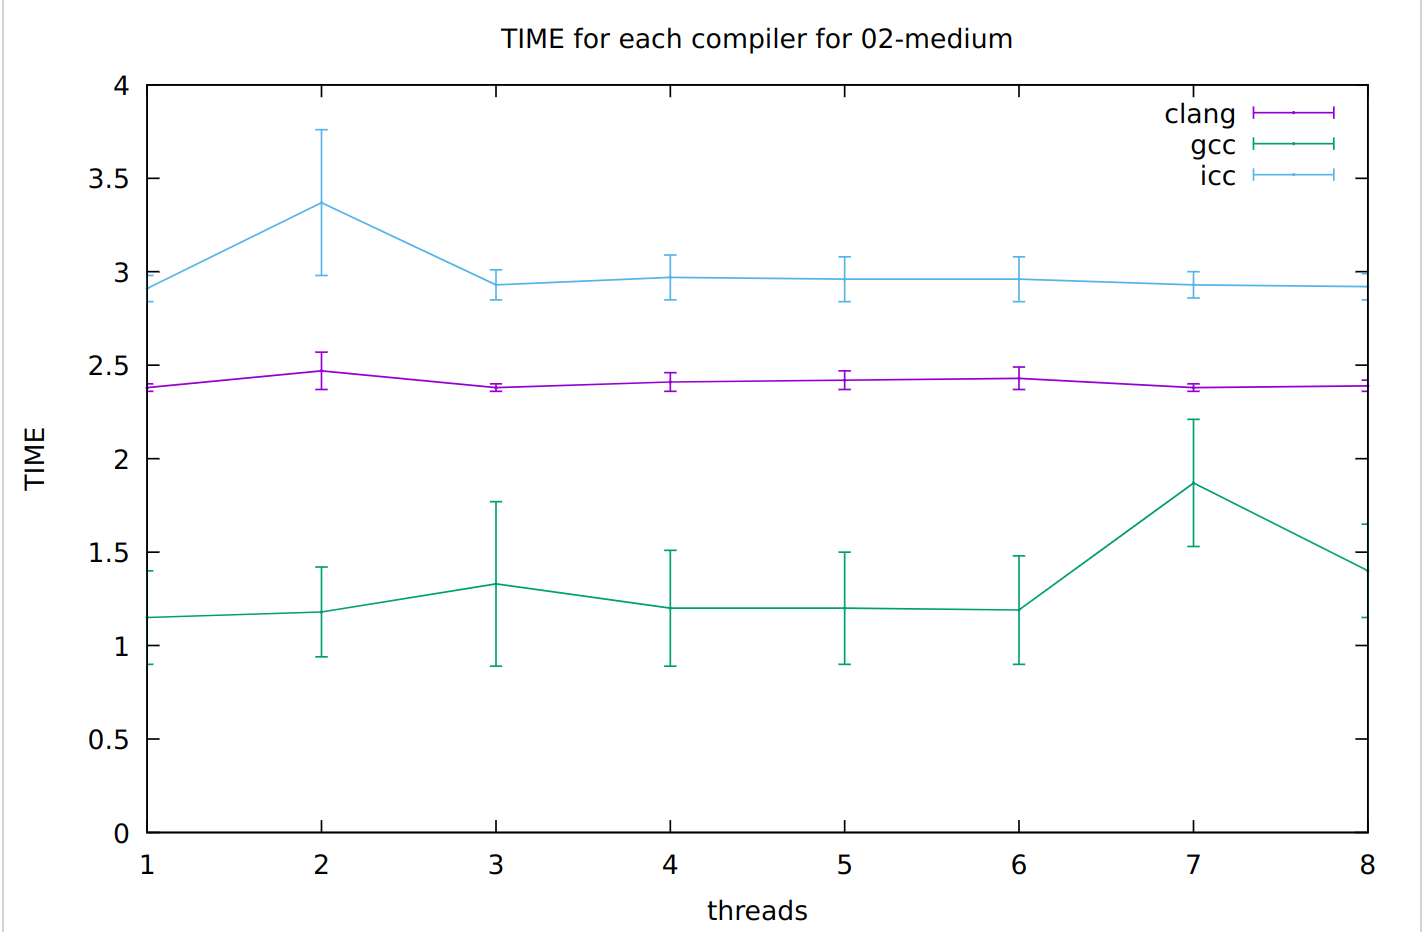
\includegraphics[width=\textwidth]{sin-cambios=02-medium}
    \end{subfigure}
    \caption{\underline{Tamaño mediano}: Tiempos de ejecución vs nº de hilos}
    \label{sin-cambios=02-medium}
\end{figure}

%%% TABLA DE TIEMPOS E IMÁGENES %%%
\begin{figure}[H]
    \centering
    \begin{subfigure}{0.4\textwidth}
        \begin{adjustbox}{width=\textwidth} 
        \begin{tabular}{|c|c|c|c|c|}
            \hline
            \rowcolor{azul} \multicolumn{2}{|c|}{}&\multicolumn{3}{c|}{\textbf{Compiler}} \\ \hline
            \rowcolor{azul} \multicolumn{2}{|c|}{}&\texttt{clang}&\texttt{gcc}&\texttt{icc}\\ \hline
            \rowcolor{azul} \textbf{Testing size} & \textbf{Threads}&\multicolumn{3}{c|}{\textbf{Average time (s)}} \\ \hline
            \multirow{8}{1cm}{\textbf{03-large}} & 1 & \(4.12\pm{0.08}\) & \(1.61\pm{0.12}\) & \(4.98\pm{0.15}\) \\ \cline{2-5}
            & 2 & \(4.10\pm{0.06}\) & \(1.61\pm{0.11}\) & \(4.94\pm{0.12}\) \\ \cline{2-5}
            & 3 & \(4.13\pm{0.09}\) & \(1.61\pm{0.12}\) & \(5.04\pm{0.20}\) \\ \cline{2-5}
            & 4 & \(4.10\pm{0.06}\) & \(1.60\pm{0.11}\) & \(4.95\pm{0.11}\) \\ \cline{2-5}
            & 5 & \(4.10\pm{0.06}\) & \(1.63\pm{0.12}\) & \(4.98\pm{0.15}\) \\ \cline{2-5}
            & 6 & \(4.16\pm{0.13}\) & \(1.60\pm{0.12}\) & \(4.94\pm{0.11}\) \\ \cline{2-5}
            & 7 & \(4.17\pm{0.11}\) & \(1.59\pm{0.12}\) & \(4.98\pm{0.15}\) \\ \cline{2-5}
            & 8 & \(4.15\pm{0.11}\) & \(1.60\pm{0.11}\) & \(4.95\pm{0.12}\) \\ \hline
        \end{tabular}
        \end{adjustbox}
    \end{subfigure}
    \hfill
    \begin{subfigure}{0.5\textwidth}
        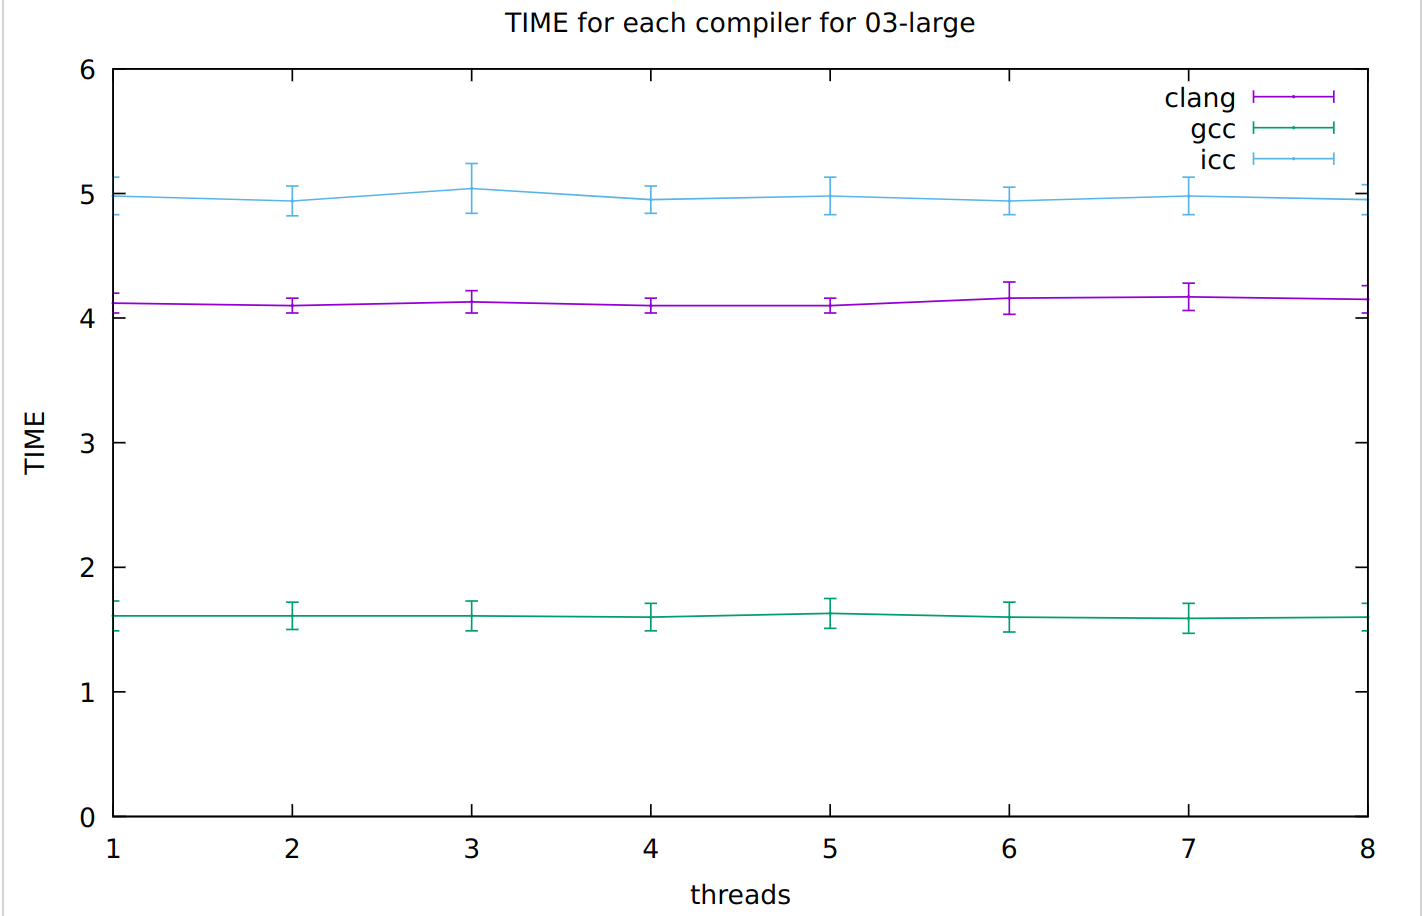
\includegraphics[width=\textwidth]{sin-cambios=03-large}
    \end{subfigure}
    \caption{\underline{Tamaño largo}: Tiempos de ejecución vs nº de hilos}
    \label{sin-cambios=03-large}
\end{figure}


\subsubsection{\textbf{1ºBucle:}}
\par El primer bucle es \texttt{while(difference / (state.height * state.width) > tolerance)}. Se podría paralelizar creando una rama master y añadiendo un pragma de tipo
\texttt{task} que comparte la variable \texttt{iterations} antes del \texttt{if(verbose)} porque la ejecución de la siguiente iteración no depende de esto.
Además, dentro de esta \texttt{task} se necesita un pragma \texttt{atomic}, porque solo un hilo puede modificar a la vez esa variable global. Esta
implementación, mostrada en el código siguiente, no ayuda mucho en el rendimiento de la aplicación y la mejora es despreciable e incluso en 
algunos casos es peor como se indica en todas las tablas y gráficas.
%%% TABLA DE TIEMPOS E IMÁGENES %%%
\begin{figure}[H]
    \centering
    \begin{subfigure}{0.4\textwidth}
        \begin{adjustbox}{width=\textwidth} 
        \begin{tabular}{|c|c|c|c|c|}
            \hline
            \rowcolor{azul} \multicolumn{2}{|c|}{}&\multicolumn{3}{c|}{\textbf{Compiler}} \\ \hline
            \rowcolor{azul} \multicolumn{2}{|c|}{}&\texttt{clang}&\texttt{gcc}&\texttt{icc}\\ \hline
            \rowcolor{azul} \textbf{Testing size} & \textbf{Threads}&\multicolumn{3}{c|}{\textbf{Average time (s)}} \\ \hline
            \multirow{8}{1cm}{\textbf{01-small}} & 1 & \(1.58\pm{0.03}\) & \(0.32\pm{0.01}\) & \(1.00\pm{0.01}\) \\ \cline{2-5}
            & 2 & \(1.58\pm{0.03}\) & \(0.32\pm{0.01}\) & \(1.02\pm{0.01}\) \\ \cline{2-5}
            & 3 & \(1.60\pm{0.03}\) & \(0.33\pm{0.01}\) & \(1.02\pm{0.01}\) \\ \cline{2-5}
            & 4 & \(1.62\pm{0.01}\) & \(0.33\pm{0.01}\) & \(1.08\pm{0.04}\) \\ \cline{2-5}
            & 5 & \(1.62\pm{0.01}\) & \(0.33\pm{0.01}\) & \(1.05\pm{0.01}\) \\ \cline{2-5}
            & 6 & \(1.72\pm{0.01}\) & \(0.46\pm{0.01}\) & \(1.41\pm{0.35}\) \\ \cline{2-5}
            & 7 & \(1.99\pm{0.01}\) & \(0.47\pm{0.01}\) & \(1.44\pm{0.32}\) \\ \cline{2-5}
            & 8 & \(1.85\pm{0.01}\) & \(0.47\pm{0.02}\) & \(1.77\pm{0.02}\) \\ \hline
        \end{tabular}
        \end{adjustbox}
    \end{subfigure}
    \hfill
    \begin{subfigure}{0.5\textwidth}
        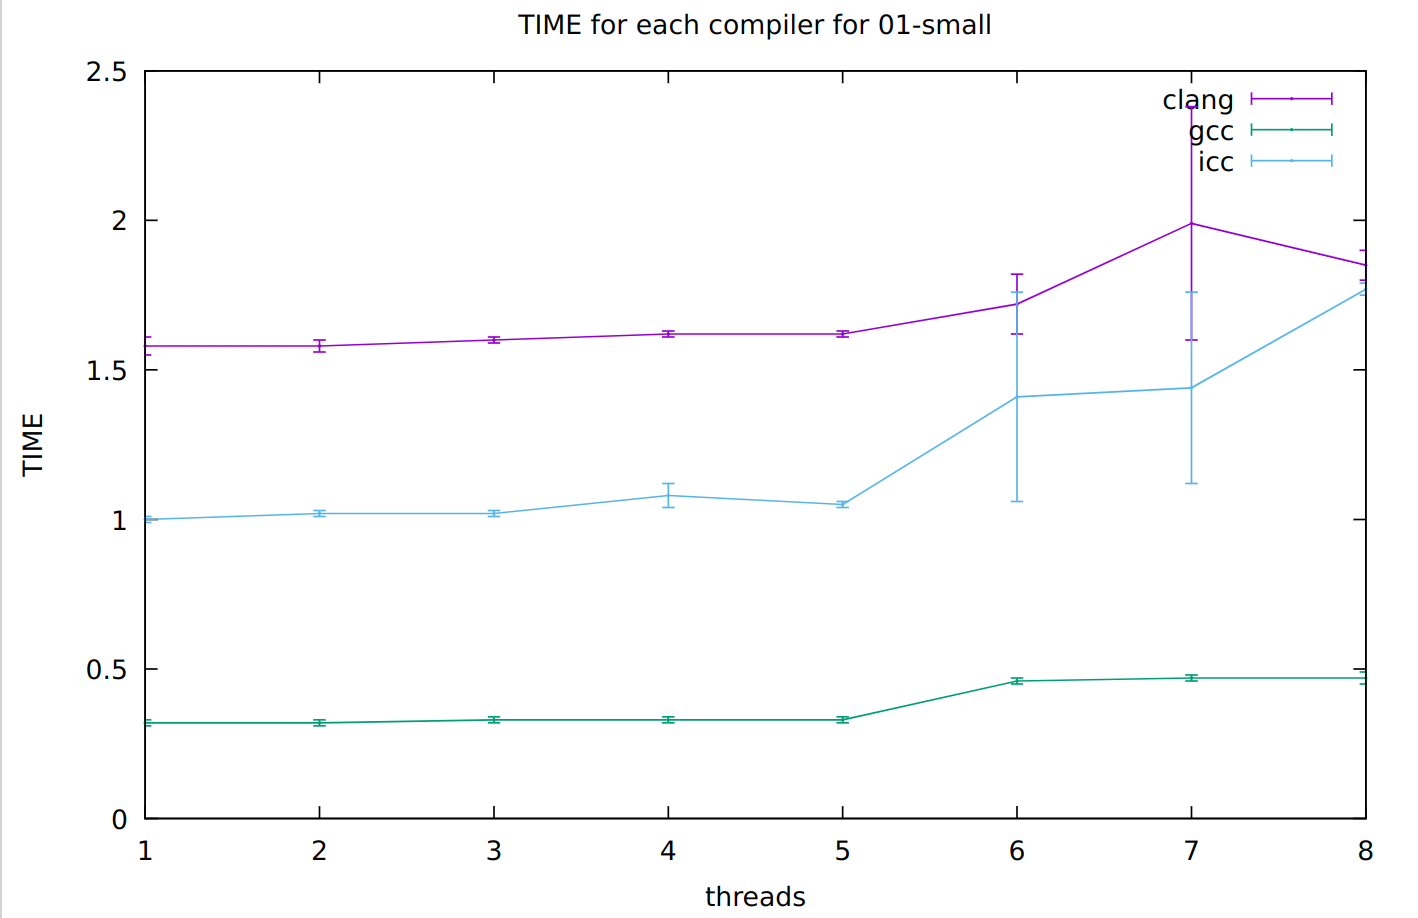
\includegraphics[width=\textwidth]{bucle1=01-small}
    \end{subfigure}
    \caption{\underline{1º Bucle, tamaño pequeño}: Tiempos de ejecución vs nº de hilos}
    \label{fig:bucle1=01-small}
\end{figure}
\newpage

\subsubsection{\textbf{heat.cpp}}
\begin{listing}[firstnumber=20]
    @@ -21,28 +21,36 @@
    void solve(Matrix<double>& state, double tolerance, int& iterations, double& last_difference) {
    Matrix<double> next_state = state;
    iterations = 0;
    double difference;
  + #pragma omp parallel
  + {
  + #pragma omp master
    do {
        difference = 0;
        for (size_t i = 1; i < state.height - 1; ++i) {
            for (size_t j = 1; j < state.width - 1; ++j) {
                next_state[i][j] = (state[i][j]
                                + state[i + 1][j]  
                                + state[i - 1][j]  
                                + state[i][j + 1]  
                                + state[i][j - 1]) / 5;
                difference = difference 
                             + abs(next_state[i][j]-state[i][j]);
            }
        }

        state.swap_data(next_state);

  + #pragma omp task shared(iterations)
  + {    
        if (verbose) {
            cout << "Iteration " << iterations << ":" << endl;
            printf_matrix("%7.3f", state);
            cout << "Difference: " << difference << endl;
        }
  + #pragma omp atomic
        ++iterations;
  + }
    } while (difference / (state.height * state.width) > tolerance);
    last_difference = difference / (state.height * state.width);
  + }
    }
\end{listing}


%%% TABLA DE TIEMPOS E IMÁGENES %%%
\begin{figure}[H]
    \centering
    \begin{subfigure}{0.4\textwidth}
        \begin{adjustbox}{width=\textwidth} 
        \begin{tabular}{|c|c|c|c|c|}
            \hline
            \rowcolor{azul} \multicolumn{2}{|c|}{}&\multicolumn{3}{c|}{\textbf{Compiler}} \\ \hline
            \rowcolor{azul} \multicolumn{2}{|c|}{}&\texttt{clang}&\texttt{gcc}&\texttt{icc}\\ \hline
            \rowcolor{azul} \textbf{Testing size} & \textbf{Threads}&\multicolumn{3}{c|}{\textbf{Average time (s)}} \\ \hline
            \multirow{8}{2.5cm}{\textbf{02-medium}} & 1 & \(4.83\pm{0.42}\) & \(0.89\pm{0.04}\) & \(2.88\pm{0.04}\) \\ \cline{2-5}
            & 2 & \(4.73\pm{0.24}\) & \(0.91\pm{0.04}\) & \(2.94\pm{0.04}\) \\ \cline{2-5}
            & 3 & \(4.57\pm{0.07}\) & \(0.90\pm{0.03}\) & \(3.22\pm{0.22}\) \\ \cline{2-5}
            & 4 & \(5.19\pm{0.57}\) & \(0.93\pm{0.04}\) & \(3.19\pm{0.21}\) \\ \cline{2-5}
            & 5 & \(4.63\pm{0.04}\) & \(1.28\pm{0.03}\) & \(3.16\pm{0.15}\) \\ \cline{2-5}
            & 6 & \(4.63\pm{0.03}\) & \(1.27\pm{0.03}\) & \(4.20\pm{0.86}\) \\ \cline{2-5}
            & 7 & \(4.64\pm{0.03}\) & \(1.27\pm{0.03}\) & \(4.83\pm{0.24}\) \\ \cline{2-5}
            & 8 & \(5.41\pm{0.08}\) & \(1.20\pm{0.04}\) & \(5.17\pm{0.10}\) \\ \hline
        \end{tabular}
        \end{adjustbox}
    \end{subfigure}
    \hfill
    \begin{subfigure}{0.5\textwidth}
        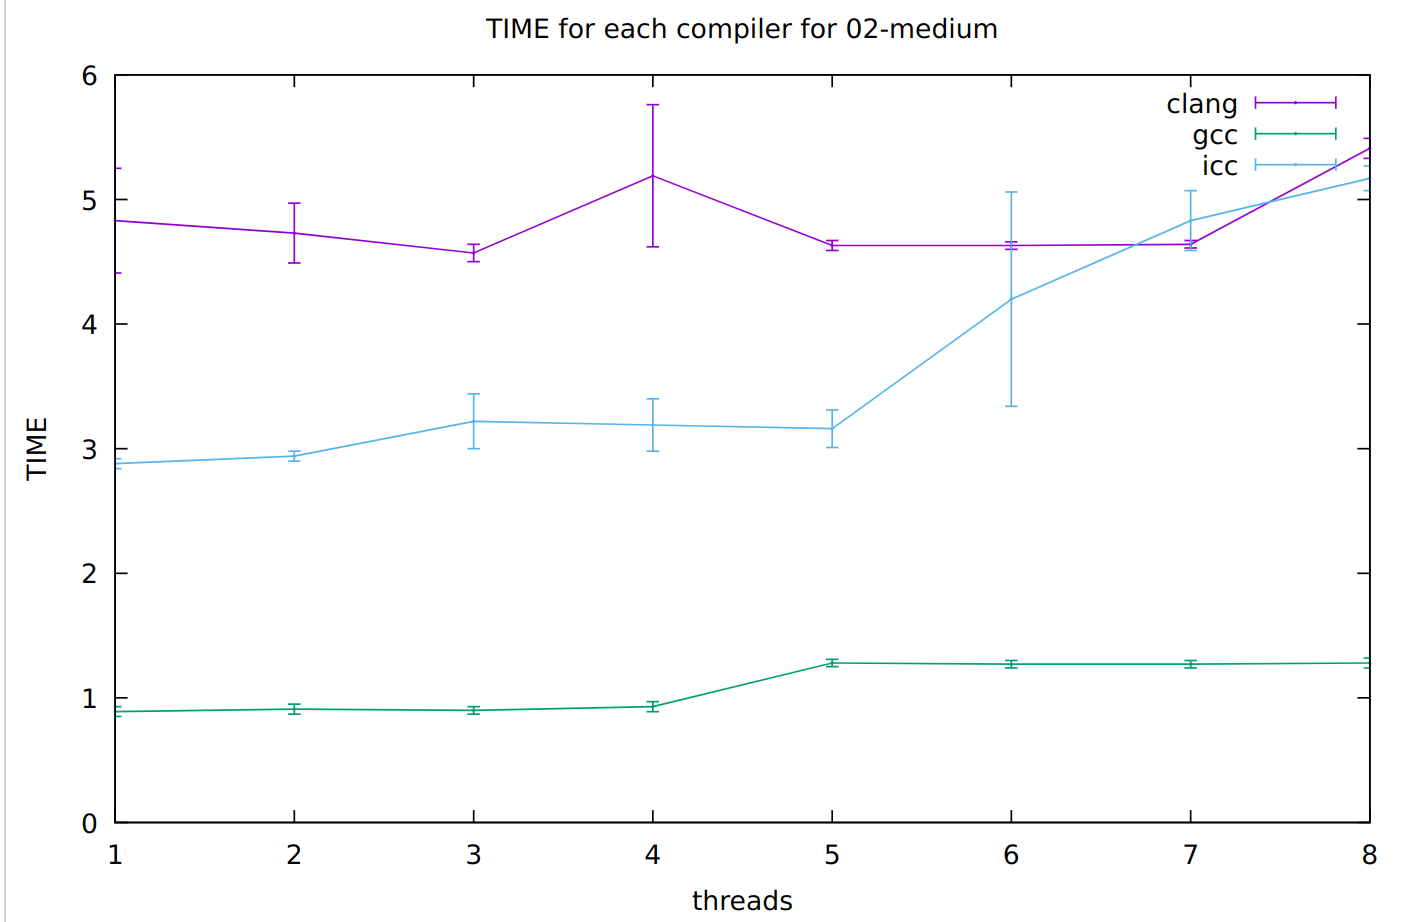
\includegraphics[width=\textwidth]{bucle1=02-medium}
    \end{subfigure}
    \caption{\underline{1º Bucle, tamaño mediano}: Tiempos de ejecución vs nº de hilos}
    \label{bucle1=02-medium}
\end{figure}

%%% TABLA DE TIEMPOS E IMÁGENES %%%
\begin{figure}[H]
    \centering
    \begin{subfigure}{0.4\textwidth}
        \begin{adjustbox}{width=\textwidth} 
        \begin{tabular}{|c|c|c|c|c|}
            \hline
            \rowcolor{azul} \multicolumn{2}{|c|}{}&\multicolumn{3}{c|}{\textbf{Compiler}} \\ \hline
            \rowcolor{azul} \multicolumn{2}{|c|}{}&\texttt{clang}&\texttt{gcc}&\texttt{icc}\\ \hline
            \rowcolor{azul} \textbf{Testing size} & \textbf{Threads}&\multicolumn{3}{c|}{\textbf{Average time (s)}} \\ \hline
            \multirow{8}{1cm}{\textbf{03-large}} & 1 & \(7.58\pm{0.01}\) & \(1.54\pm{0.11}\) & \(4.97\pm{0.13}\) \\ \cline{2-5}
            & 2 & \(7.69\pm{0.05}\) & \(1.55\pm{0.07}\) & \(5.11\pm{0.16}\) \\ \cline{2-5}
            & 3 & \(7.83\pm{0.01}\) & \(1.56\pm{0.08}\) & \(5.20\pm{0.21}\) \\ \cline{2-5}
            & 4 & \(7.87\pm{0.06}\) & \(1.61\pm{0.09}\) & \(5.23\pm{0.16}\) \\ \cline{2-5}
            & 5 & \(7.90\pm{0.03}\) & \(2.19\pm{0.05}\) & \(5.23\pm{0.18}\) \\ \cline{2-5}
            & 6 & \(7.87\pm{0.05}\) & \(2.17\pm{0.05}\) & \(5.20\pm{0.14}\) \\ \cline{2-5}
            & 7 & \(8.86\pm{0.01}\) & \(2.16\pm{0.06}\) & \(8.78\pm{0.18}\) \\ \cline{2-5}
            & 8 & \(8.85\pm{0.03}\) & \(2.15\pm{0.03}\) & \(8.76\pm{0.15}\) \\ \hline
        \end{tabular}
        \end{adjustbox}
    \end{subfigure}
    \hfill
    \begin{subfigure}{0.5\textwidth}
        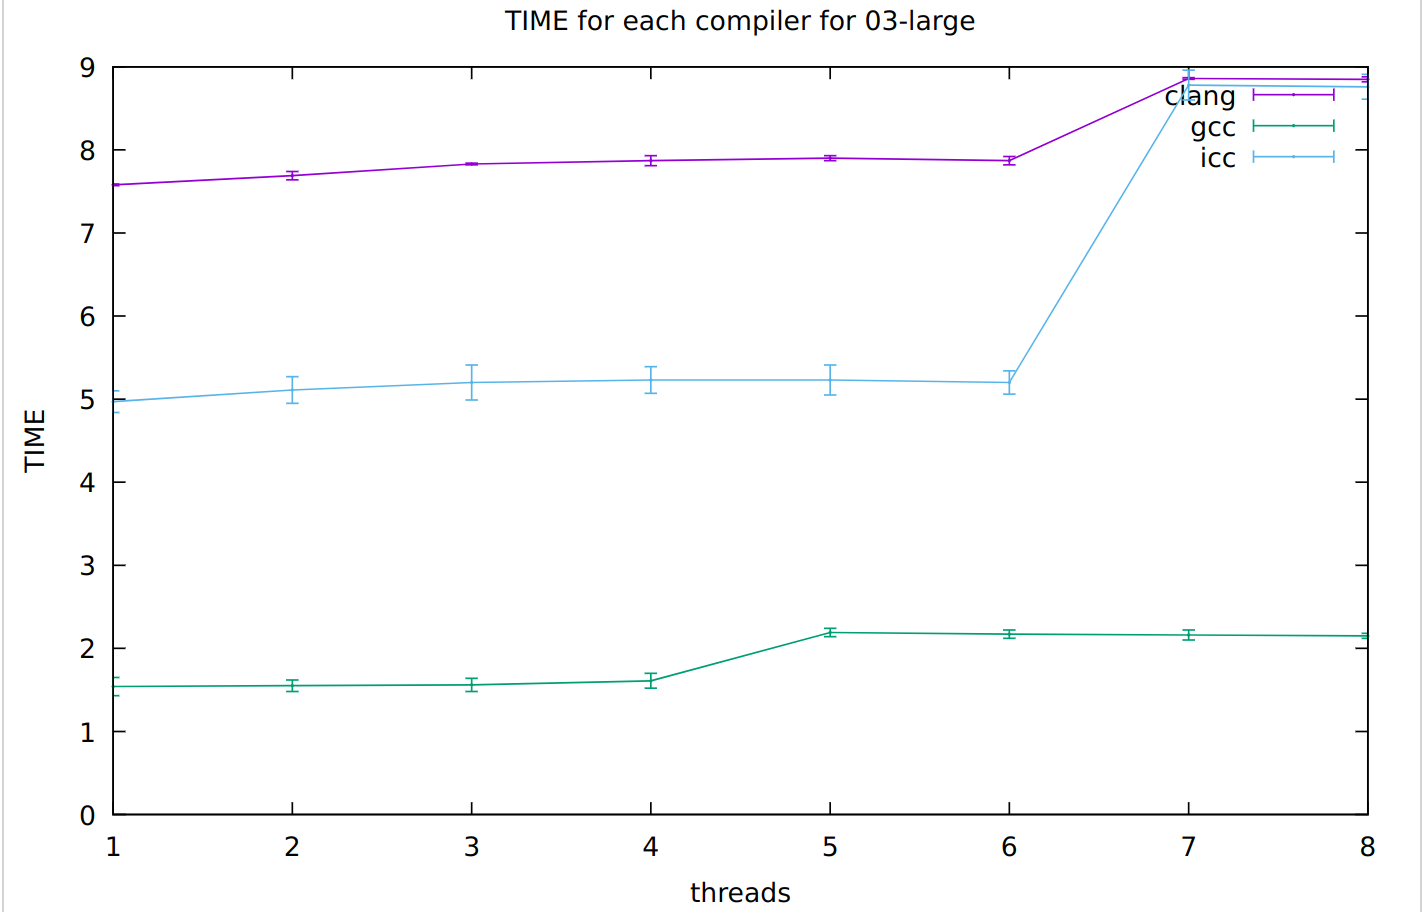
\includegraphics[width=\textwidth]{bucle1=03-large}
    \end{subfigure}
    \caption{\underline{1º Bucle, tamaño largo}: Tiempos de ejecución vs nº de hilos}
    \label{bucle1=03-large}
\end{figure}

\subsubsection{\textbf{2ºBucle:}}

\par El segundo es el bucle exterior \texttt{for (size\_t i = 1; i < state.height - 1; ++i)}, es el mejor candidato para paralelizar, hay que añadir un
pragma \texttt{\#pragma omp parallel for reduction (max:difference)} para que ejecute las instrucciones en paralelo pero tenga en cuenta la
instrucción max que no deben de ejecutarla dos hilos a la vez.

%%% TABLA DE TIEMPOS E IMÁGENES %%%
\begin{figure}[H]
    \centering
    \begin{subfigure}{0.4\textwidth}
        \begin{adjustbox}{width=\textwidth} 
        \begin{tabular}{|c|c|c|c|c|}
            \hline
            \rowcolor{azul} \multicolumn{2}{|c|}{}&\multicolumn{3}{c|}{\textbf{Compiler}} \\ \hline
            \rowcolor{azul} \multicolumn{2}{|c|}{}&\texttt{clang}&\texttt{gcc}&\texttt{icc}\\ \hline
            \rowcolor{azul} \textbf{Testing size} & \textbf{Threads}&\multicolumn{3}{c|}{\textbf{Average time (s)}} \\ \hline
            \multirow{8}{1cm}{\textbf{01-small}} & 1 & \(1.53\pm{0.00}\) & \(0.36\pm{0.00}\) & \(1.01\pm{0.01}\) \\ \cline{2-5}
            & 2 & \(0.81\pm{0.02}\) & \(0.18\pm{0.01}\) & \(0.53\pm{0.01}\) \\ \cline{2-5}
            & 3 & \(0.54\pm{0.00}\) & \(0.13\pm{0.01}\) & \(0.37\pm{0.00}\) \\ \cline{2-5}
            & 4 & \(0.42\pm{0.00}\) & \(0.12\pm{0.03}\) & \(0.34\pm{0.05}\) \\ \cline{2-5}
            & 5 & \(0.41\pm{0.01}\) & \(0.14\pm{0.01}\) & \(0.45\pm{0.01}\) \\ \cline{2-5}
            & 6 & \(0.35\pm{0.01}\) & \(0.13\pm{0.02}\) & \(0.40\pm{0.03}\) \\ \cline{2-5}
            & 7 & \(0.31\pm{0.01}\) & \(0.11\pm{0.00}\) & \(0.33\pm{0.01}\) \\ \cline{2-5}
            & 8 & \(0.29\pm{0.01}\) & \(0.11\pm{0.00}\) & \(0.33\pm{0.02}\) \\ \hline
        \end{tabular}
        \end{adjustbox}
    \end{subfigure}
    \hfill
    \begin{subfigure}{0.5\textwidth}
        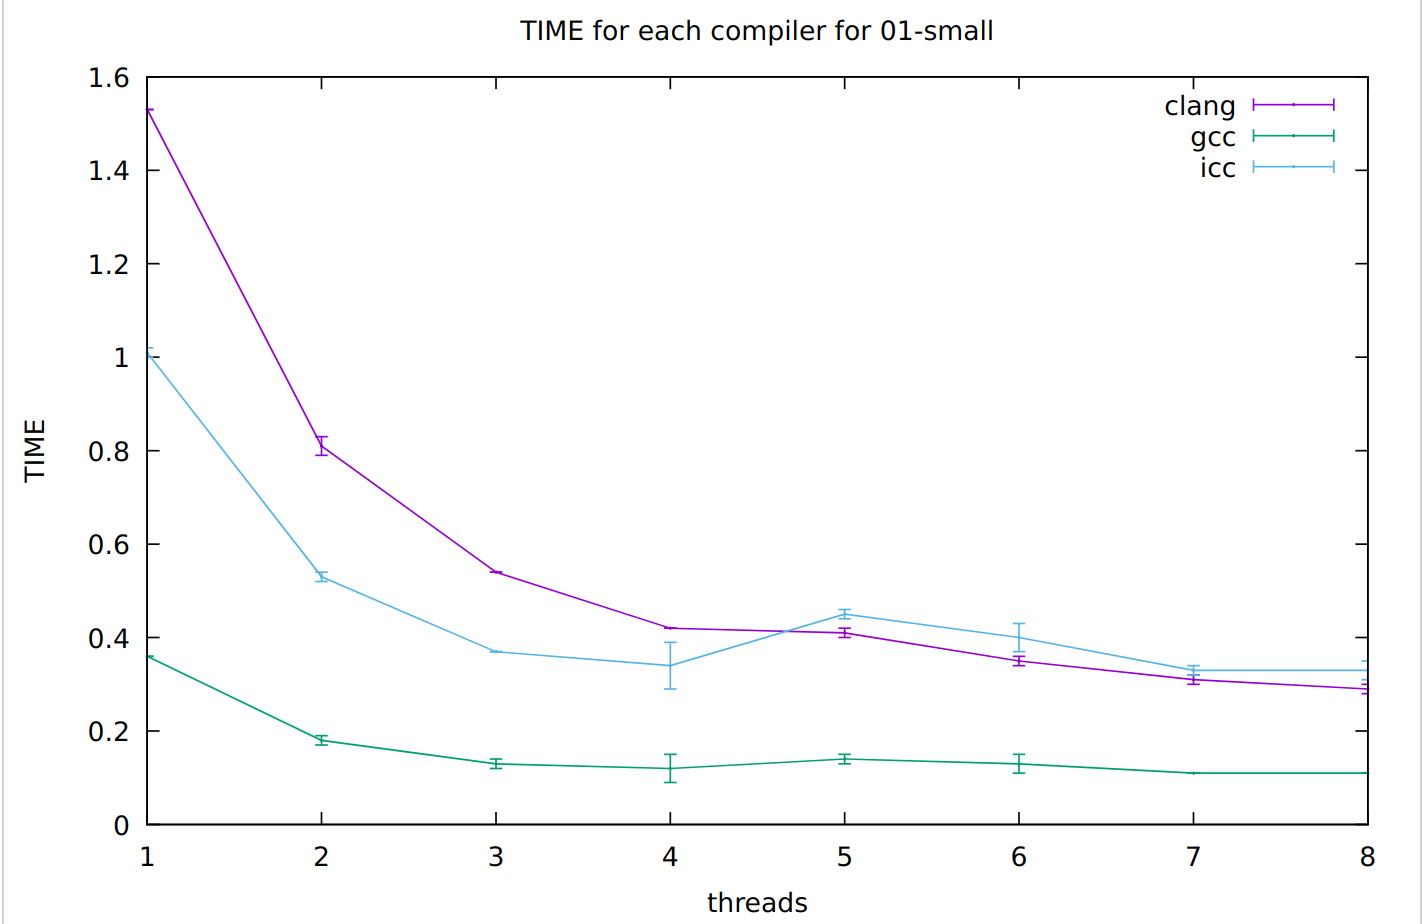
\includegraphics[width=\textwidth]{bucle2=01-small}
    \end{subfigure}
    \caption{\underline{Tamaño pequeño}: Tiempos de ejecución vs nº de hilos}
    \label{fig:bucle2=01-small}
\end{figure}

%%% TABLA DE TIEMPOS E IMÁGENES %%%
\begin{figure}[H]
    \centering
    \begin{subfigure}{0.4\textwidth}
        \begin{adjustbox}{width=\textwidth} 
        \begin{tabular}{|c|c|c|c|c|}
            \hline
            \rowcolor{azul} \multicolumn{2}{|c|}{}&\multicolumn{3}{c|}{\textbf{Compiler}} \\ \hline
            \rowcolor{azul} \multicolumn{2}{|c|}{}&\texttt{clang}&\texttt{gcc}&\texttt{icc}\\ \hline
            \rowcolor{azul} \textbf{Testing size} & \textbf{Threads}&\multicolumn{3}{c|}{\textbf{Average time (s)}} \\ \hline
            \multirow{8}{2.5cm}{\textbf{02-medium}} & 1 & \(4.45\pm{0.03}\) & \(0.89\pm{0.03}\) & \(2.90\pm{0.03}\) \\ \cline{2-5}
            & 2 & \(2.31\pm{0.05}\) & \(0.47\pm{0.02}\) & \(3.37\pm{0.06}\) \\ \cline{2-5}
            & 3 & \(1.52\pm{0.00}\) & \(0.33\pm{0.02}\) & \(2.93\pm{0.05}\) \\ \cline{2-5}
            & 4 & \(1.20\pm{0.03}\) & \(0.30\pm{0.06}\) & \(2.97\pm{0.03}\) \\ \cline{2-5}
            & 5 & \(1.16\pm{0.04}\) & \(0.37\pm{0.02}\) & \(2.96\pm{0.02}\) \\ \cline{2-5}
            & 6 & \(0.97\pm{0.03}\) & \(0.31\pm{0.01}\) & \(2.96\pm{0.07}\) \\ \cline{2-5}
            & 7 & \(0.87\pm{0.05}\) & \(0.27\pm{0.01}\) & \(2.93\pm{0.02}\) \\ \cline{2-5}
            & 8 & \(0.77\pm{0.03}\) & \(0.25\pm{0.01}\) & \(2.92\pm{0.01}\) \\ \hline
        \end{tabular}
        \end{adjustbox}
    \end{subfigure}
    \hfill
    \begin{subfigure}{0.5\textwidth}
        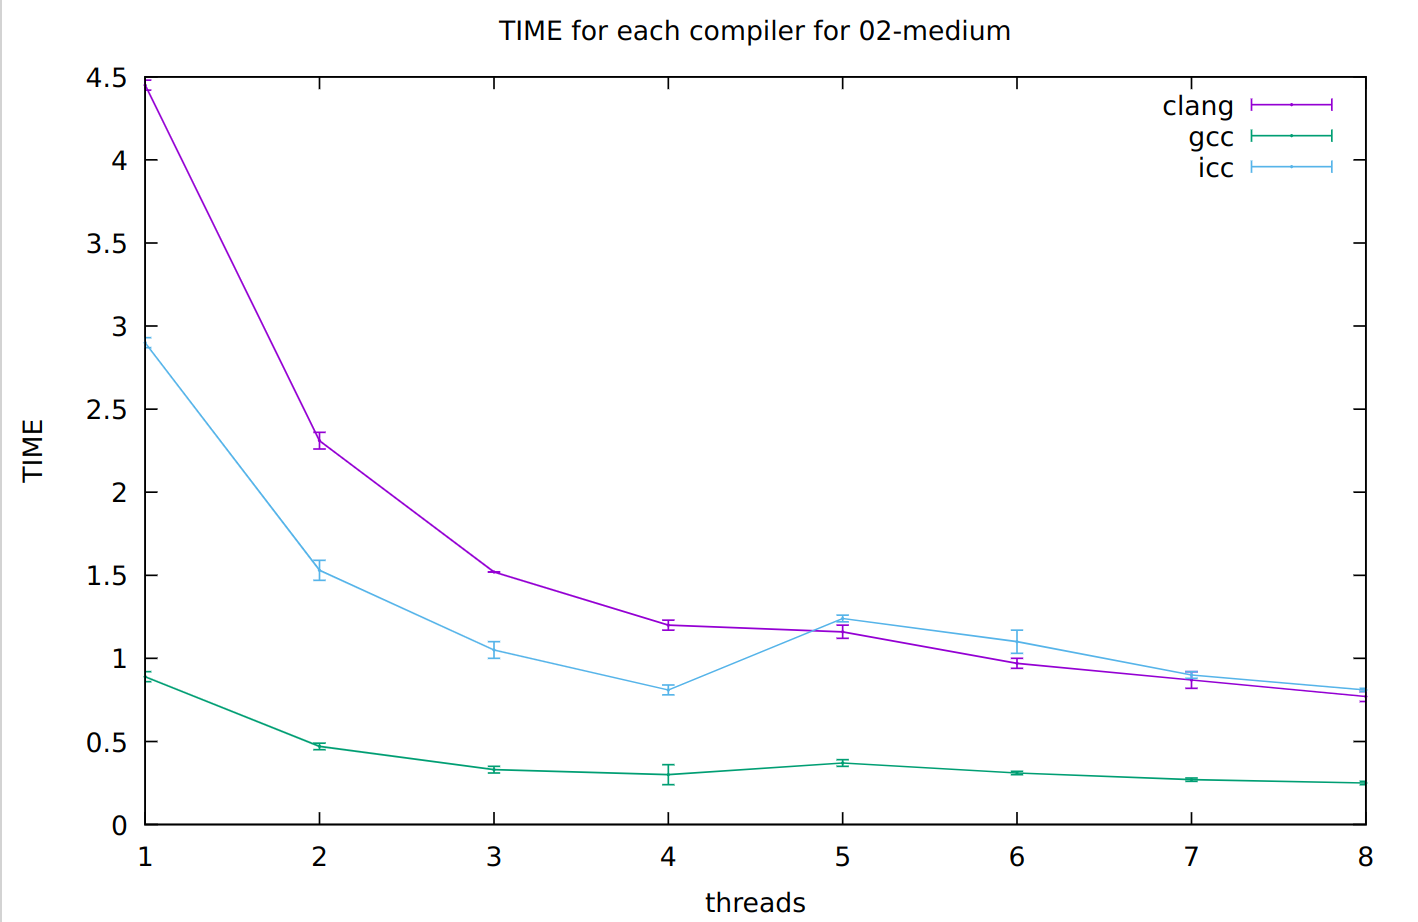
\includegraphics[width=\textwidth]{bucle2=02-medium}
    \end{subfigure}
    \caption{\underline{Tamaño mediano}: Tiempos de ejecución vs nº de hilos}
    \label{bucle2=02-medium}
\end{figure}

%%% TABLA DE TIEMPOS E IMÁGENES %%%
\begin{figure}[H]
    \centering
    \begin{subfigure}{0.4\textwidth}
        \begin{adjustbox}{width=\textwidth} 
        \begin{tabular}{|c|c|c|c|c|}
            \hline
            \rowcolor{azul} \multicolumn{2}{|c|}{}&\multicolumn{3}{c|}{\textbf{Compiler}} \\ \hline
            \rowcolor{azul} \multicolumn{2}{|c|}{}&\texttt{clang}&\texttt{gcc}&\texttt{icc}\\ \hline
            \rowcolor{azul} \textbf{Testing size} & \textbf{Threads}&\multicolumn{3}{c|}{\textbf{Average time (s)}} \\ \hline
            \multirow{8}{1cm}{\textbf{03-large}} & 1 & \(7.62\pm{0.15}\) & \(1.56\pm{0.07}\) & \(5.00\pm{0.12}\) \\ \cline{2-5}
            & 2 & \(3.93\pm{0.05}\) & \(0.80\pm{0.04}\) & \(2.63\pm{0.11}\) \\ \cline{2-5}
            & 3 & \(2.65\pm{0.02}\) & \(0.55\pm{0.04}\) & \(1.85\pm{0.15}\) \\ \cline{2-5}
            & 4 & \(2.02\pm{0.02}\) & \(0.42\pm{0.02}\) & \(1.37\pm{0.05}\) \\ \cline{2-5}
            & 5 & \(1.97\pm{0.12}\) & \(0.60\pm{0.03}\) & \(2.10\pm{0.02}\) \\ \cline{2-5}
            & 6 & \(1.67\pm{0.09}\) & \(0.51\pm{0.02}\) & \(1.78\pm{0.05}\) \\ \cline{2-5}
            & 7 & \(1.43\pm{0.07}\) & \(0.47\pm{0.04}\) & \(1.51\pm{0.02}\) \\ \cline{2-5}
            & 8 & \(1.28\pm{0.06}\) & \(0.41\pm{0.02}\) & \(1.40\pm{0.05}\) \\ \hline
        \end{tabular}
        \end{adjustbox}
    \end{subfigure}
    \hfill
    \begin{subfigure}{0.5\textwidth}
        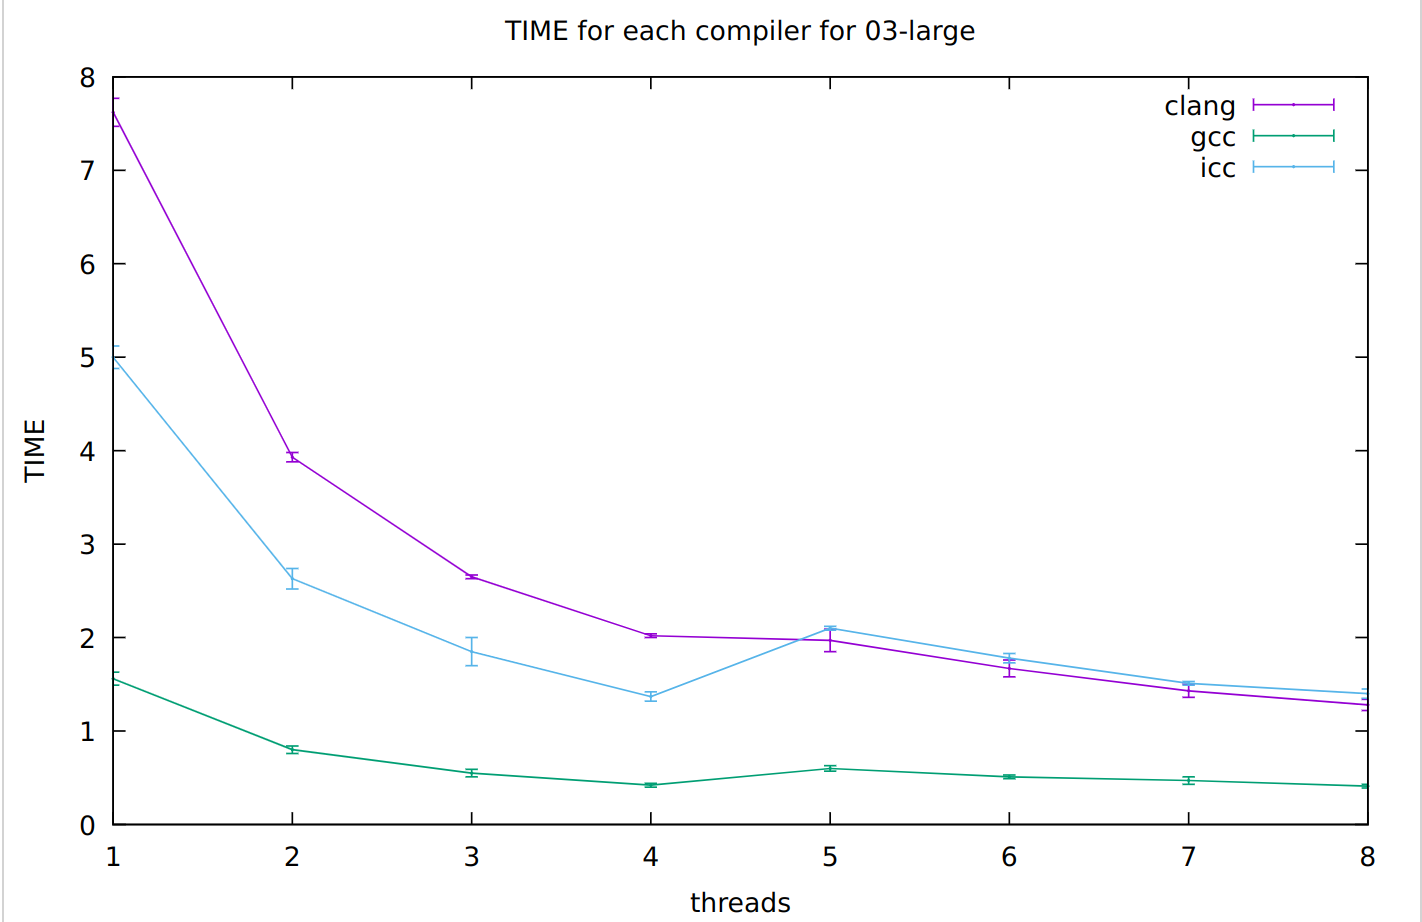
\includegraphics[width=\textwidth]{bucle2=03-large}
    \end{subfigure}
    \caption{\underline{Tamaño largo}: Tiempos de ejecución vs nº de hilos}
    \label{bucle2=03-large}
\end{figure}
\subsubsection{\textbf{3ºBucle:}}
\begin{listing}
    @@ -20,3 +20,4 @@
\end{listing}

\subsubsection{\textbf{Paralelización de los tres bucles:}}

%%% TABLA DE TIEMPOS E IMÁGENES %%%
\begin{figure}[H]
    \centering
    \begin{subfigure}{0.4\textwidth}
        \begin{adjustbox}{width=\textwidth} 
        \begin{tabular}{|c|c|c|c|c|}
            \hline
            \rowcolor{azul} \multicolumn{2}{|c|}{}&\multicolumn{3}{c|}{\textbf{Compiler}} \\ \hline
            \rowcolor{azul} \multicolumn{2}{|c|}{}&\texttt{clang}&\texttt{gcc}&\texttt{icc}\\ \hline
            \rowcolor{azul} \textbf{Testing size} & \textbf{Threads}&\multicolumn{3}{c|}{\textbf{Average time (s)}} \\ \hline
            \multirow{8}{1cm}{\textbf{01-small}} & 1 & \(1.53\pm{0.00}\) & \(0.38\pm{0.01}\) & \(1.01\pm{0.0}\) \\ \cline{2-5}
            & 2 & \(1.56\pm{0.00}\) & \(0.35\pm{0.01}\) & \(1.03\pm{0.01}\) \\ \cline{2-5}
            & 3 & \(1.58\pm{0.00}\) & \(0.34\pm{0.02}\) & \(1.06\pm{0.05}\) \\ \cline{2-5}
            & 4 & \(1.60\pm{0.00}\) & \(0.34\pm{0.02}\) & \(1.08\pm{0.01}\) \\ \cline{2-5}
            & 5 & \(1.73\pm{0.12}\) & \(0.47\pm{0.01}\) & \(1.42\pm{0.35}\) \\ \cline{2-5}
            & 6 & \(1.70\pm{0.10}\) & \(0.48\pm{0.01}\) & \(1.42\pm{0.35}\) \\ \cline{2-5}
            & 7 & \(1.73\pm{0.08}\) & \(0.48\pm{0.01}\) & \(1.46\pm{0.41}\) \\ \cline{2-5}
            & 8 & \(1.83\pm{0.02}\) & \(0.47\pm{0.01}\) & \(1.79\pm{0.02}\) \\ \hline
        \end{tabular}
        \end{adjustbox}
    \end{subfigure}
    \hfill
    \begin{subfigure}{0.5\textwidth}
        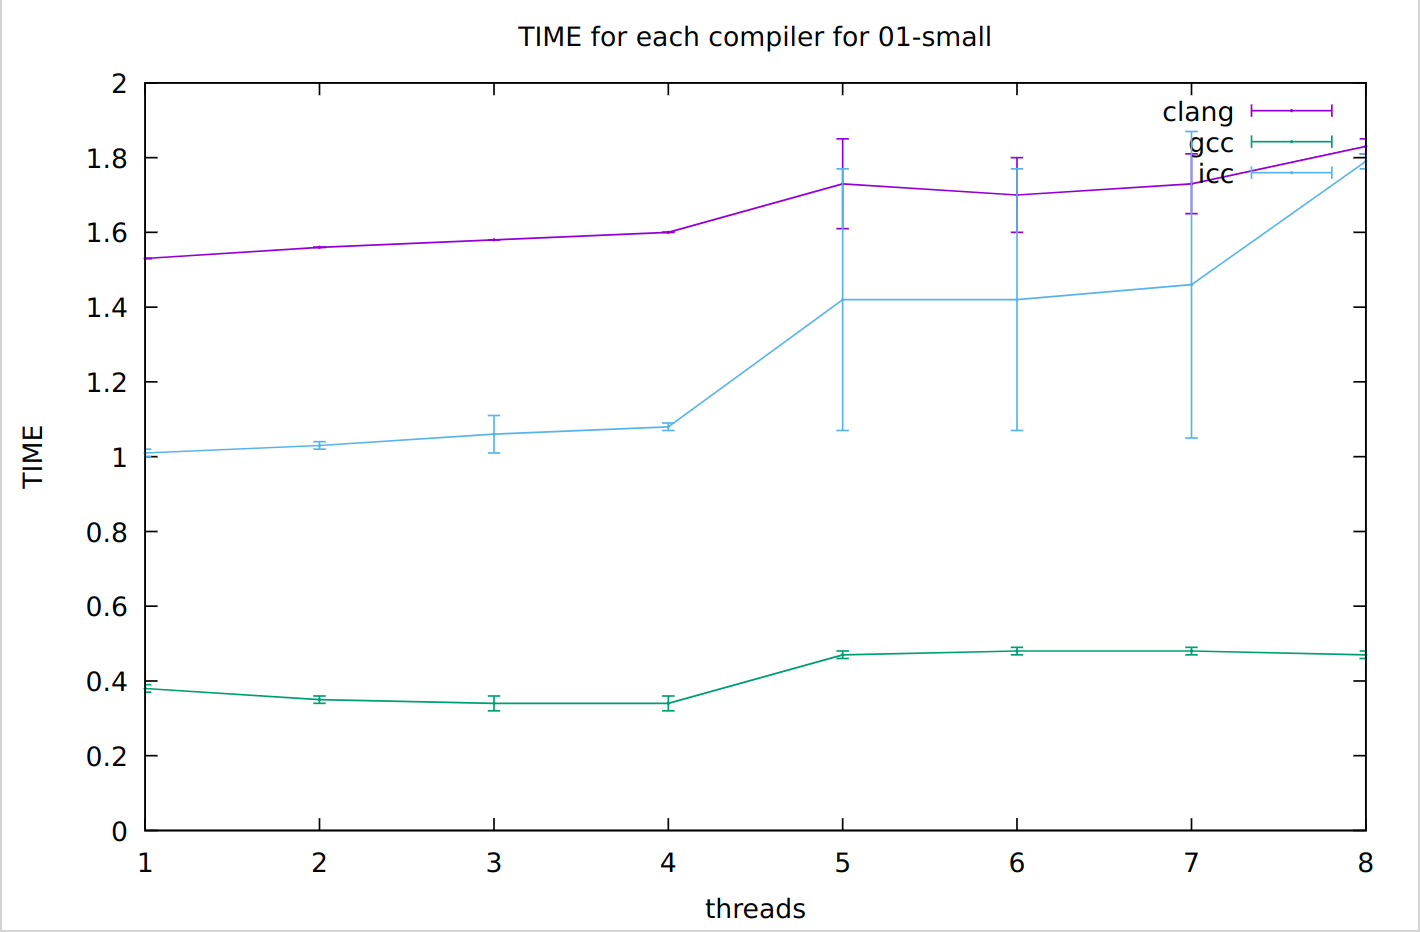
\includegraphics[width=\textwidth]{bucle1-2=01-small}
    \end{subfigure}
    \caption{\underline{Tamaño pequeño}: Tiempos de ejecución vs nº de hilos}
    \label{fig:bucle1-2=01-small}
\end{figure}

%%% TABLA DE TIEMPOS E IMÁGENES %%%
\begin{figure}[H]
    \centering
    \begin{subfigure}{0.4\textwidth}
        \begin{adjustbox}{width=\textwidth} 
        \begin{tabular}{|c|c|c|c|c|}
            \hline
            \rowcolor{azul} \multicolumn{2}{|c|}{}&\multicolumn{3}{c|}{\textbf{Compiler}} \\ \hline
            \rowcolor{azul} \multicolumn{2}{|c|}{}&\texttt{clang}&\texttt{gcc}&\texttt{icc}\\ \hline
            \rowcolor{azul} \textbf{Testing size} & \textbf{Threads}&\multicolumn{3}{c|}{\textbf{Average time (s)}} \\ \hline
            \multirow{8}{2.5cm}{\textbf{02-medium}} & 1 & \(4.50\pm{0.09}\) & \(0.88\pm{0.04}\) & \(2.94\pm{0.08}\) \\ \cline{2-5}
            & 2 & \(4.54\pm{0.03}\) & \(0.91\pm{0.04}\) & \(2.96\pm{0.04}\) \\ \cline{2-5}
            & 3 & \(4.53\pm{0.01}\) & \(0.91\pm{0.04}\) & \(2.97\pm{0.05}\) \\ \cline{2-5}
            & 4 & \(4.64\pm{0.02}\) & \(0.93\pm{0.04}\) & \(3.02\pm{0.04}\) \\ \cline{2-5}
            & 5 & \(4.68\pm{0.05}\) & \(0.94\pm{0.04}\) & \(3.03\pm{0.04}\) \\ \cline{2-5}
            & 6 & \(5.20\pm{0.02}\) & \(1.31\pm{0.03}\) & \(3.03\pm{0.04}\) \\ \cline{2-5}
            & 7 & \(5.25\pm{0.04}\) & \(1.30\pm{0.02}\) & \(5.15\pm{0.05}\) \\ \cline{2-5}
            & 8 & \(5.21\pm{0.00}\) & \(1.31\pm{0.03}\) & \(5.13\pm{0.06}\) \\ \hline
        \end{tabular}
        \end{adjustbox}
    \end{subfigure}
    \hfill
    \begin{subfigure}{0.5\textwidth}
        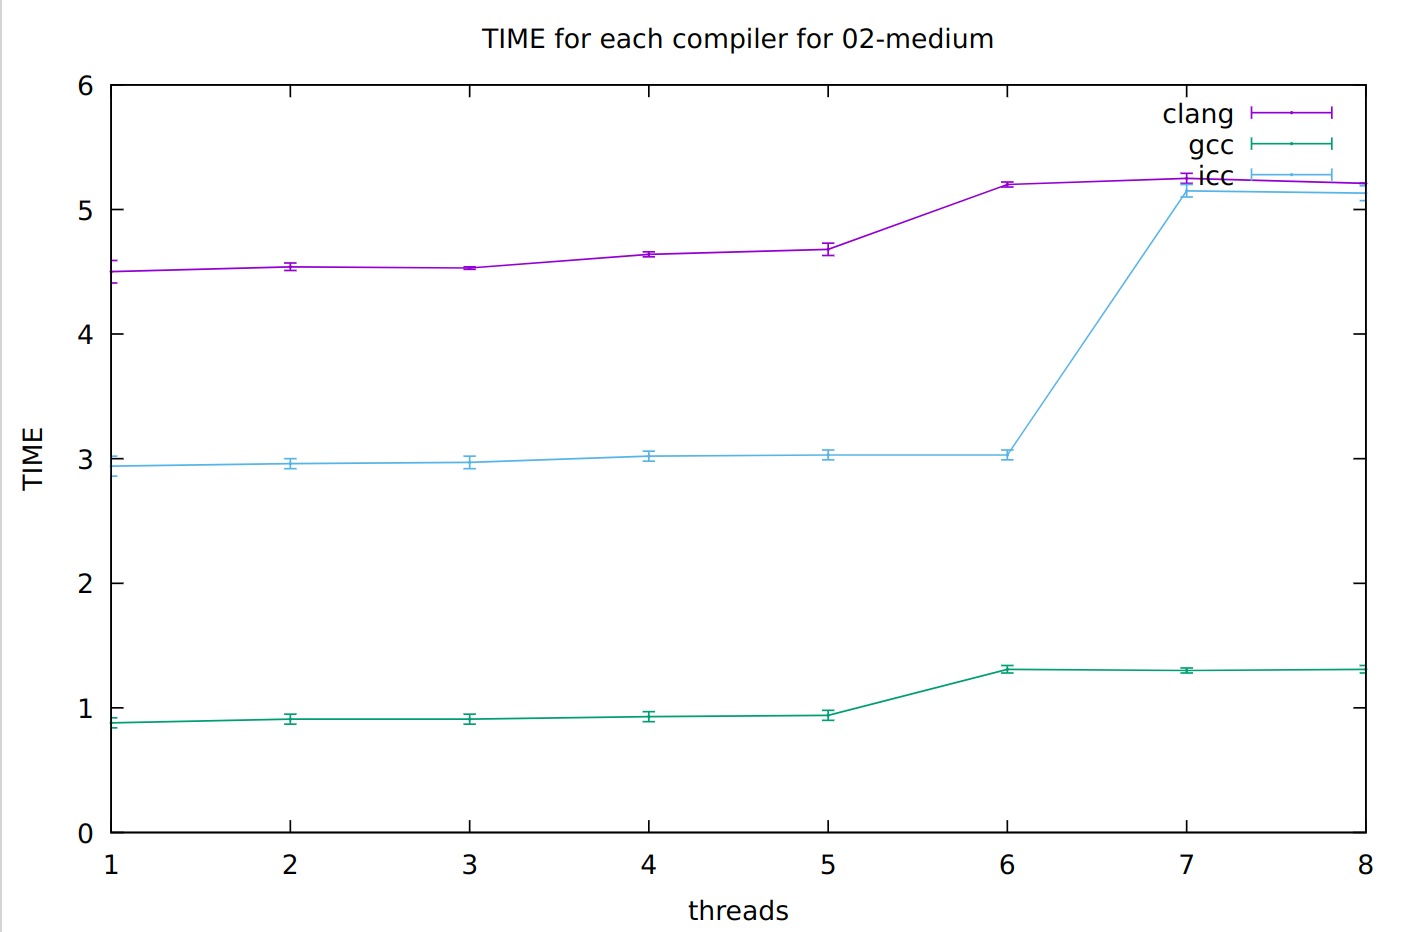
\includegraphics[width=\textwidth]{bucle1-2=02-medium}
    \end{subfigure}
    \caption{\underline{Tamaño mediano}: Tiempos de ejecución vs nº de hilos}
    \label{bucle1-2=02-medium}
\end{figure}

%%% TABLA DE TIEMPOS E IMÁGENES %%%
\begin{figure}[H]
    \centering
    \begin{subfigure}{0.4\textwidth}
        \begin{adjustbox}{width=\textwidth} 
        \begin{tabular}{|c|c|c|c|c|}
            \hline
            \rowcolor{azul} \multicolumn{2}{|c|}{}&\multicolumn{3}{c|}{\textbf{Compiler}} \\ \hline
            \rowcolor{azul} \multicolumn{2}{|c|}{}&\texttt{clang}&\texttt{gcc}&\texttt{icc}\\ \hline
            \rowcolor{azul} \textbf{Testing size} & \textbf{Threads}&\multicolumn{3}{c|}{\textbf{Average time (s)}} \\ \hline
            \multirow{8}{1cm}{\textbf{03-large}} & 1 & \(7.56\pm{0.02}\) & \(1.53\pm{0.08}\) & \(5.00\pm{0.11}\) \\ \cline{2-5}
            & 2 & \(7.78\pm{0.01}\) & \(1.57\pm{0.08}\) & \(5.07\pm{0.10}\) \\ \cline{2-5}
            & 3 & \(7.80\pm{0.04}\) & \(1.57\pm{0.08}\) & \(5.18\pm{0.21}\) \\ \cline{2-5}
            & 4 & \(7.92\pm{0.06}\) & \(1.61\pm{0.07}\) & \(5.22\pm{0.12}\) \\ \cline{2-5}
            & 5 & \(7.85\pm{0.02}\) & \(2.20\pm{0.04}\) & \(5.31\pm{0.19}\) \\ \cline{2-5}
            & 6 & \(8.89\pm{0.06}\) & \(1.62\pm{0.07}\) & \(5.16\pm{0.09}\) \\ \cline{2-5}
            & 7 & \(8.90\pm{0.02}\) & \(2.21\pm{0.04}\) & \(8.71\pm{0.04}\) \\ \cline{2-5}
            & 8 & \(8.83\pm{0.03}\) & \(2.21\pm{0.04}\) & \(8.75\pm{0.14}\) \\ \hline
        \end{tabular}
        \end{adjustbox}
    \end{subfigure}
    \hfill
    \begin{subfigure}{0.5\textwidth}
        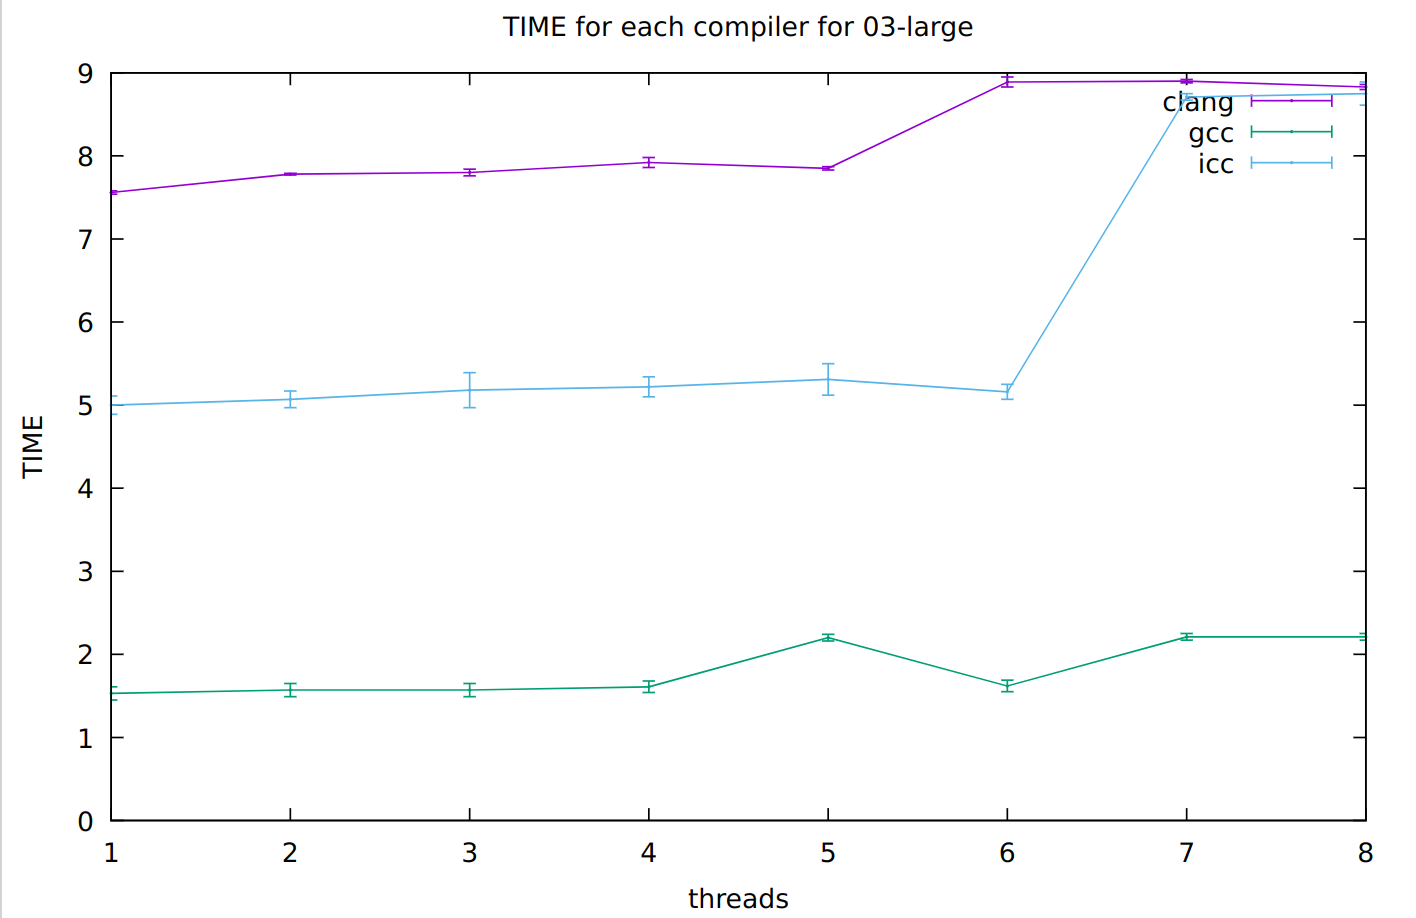
\includegraphics[width=\textwidth]{bucle1-2=03-large}
    \end{subfigure}
    \caption{\underline{Tamaño largo}: Tiempos de ejecución vs nº de hilos}
    \label{bucle1-2=03-large}
\end{figure}

%%%%%%%%%%%%%%%%%%%%%%%%%%%%%%%%%%%%%%%%%%%%%%%%%%%%%%%%%%%%%%%%%%%%%%%%%%%%%%%%%
%%% TABLA DE TIEMPOS E IMÁGENES %%%
\begin{figure}[H]
    \centering
    \begin{subfigure}{0.4\textwidth}
        \begin{adjustbox}{width=\textwidth} 
        \begin{tabular}{|c|c|c|c|c|}
            \hline
            \rowcolor{azul} \multicolumn{2}{|c|}{}&\multicolumn{3}{c|}{\textbf{Compiler}} \\ \hline
            \rowcolor{azul} \multicolumn{2}{|c|}{}&\texttt{clang}&\texttt{gcc}&\texttt{icc}\\ \hline
            \rowcolor{azul} \textbf{Testing size} & \textbf{Threads}&\multicolumn{3}{c|}{\textbf{Average time (s)}} \\ \hline
            \multirow{8}{1cm}{\textbf{01-small}} & 1 & \(3.36\pm{0.02}\) & \(1.80\pm{0.38}\) & \(5.68\pm{0.01}\) \\ \cline{2-5}
            & 2 & \(1.74\pm{0.01}\) & \(0.72\pm{0.01}\) & \(2.93\pm{0.01}\) \\ \cline{2-5}
            & 3 & \(1.19\pm{0.02}\) & \(0.50\pm{0.01}\) & \(1.98\pm{0.01}\) \\ \cline{2-5}
            & 4 & \(0.91\pm{0.01}\) & \(0.39\pm{0.01}\) & \(1.52\pm{0.01}\) \\ \cline{2-5}
            & 5 & \(1.35\pm{0.00}\) & \(0.59\pm{0.00}\) & \(2.21\pm{0.00}\) \\ \cline{2-5}
            & 6 & \(1.13\pm{0.00}\) & \(0.49\pm{0.00}\) & \(1.85\pm{0.01}\) \\ \cline{2-5}
            & 7 & \(0.98\pm{0.01}\) & \(0.43\pm{0.00}\) & \(1.60\pm{0.01}\) \\ \cline{2-5}
            & 8 & \(0.87\pm{0.00}\) & \(0.40\pm{0.01}\) & \(1.44\pm{0.03}\) \\ \hline
        \end{tabular}
        \end{adjustbox}
    \end{subfigure}
    \hfill
    \begin{subfigure}{0.5\textwidth}
        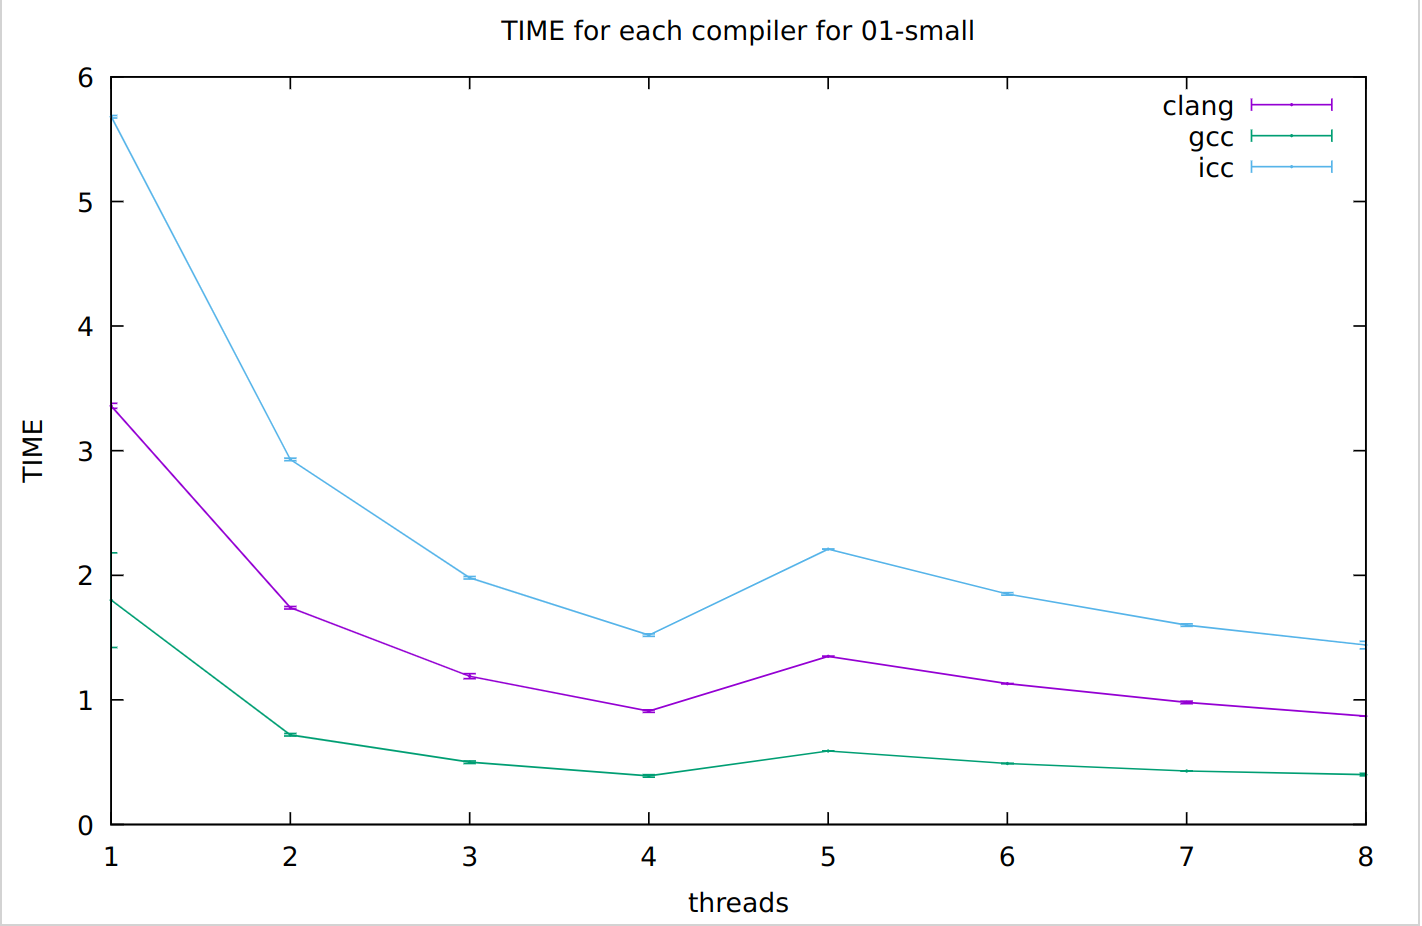
\includegraphics[width=\textwidth]{bucle2-3=01-small}
    \end{subfigure}
    \caption{\underline{Tamaño pequeño}: Tiempos de ejecución vs nº de hilos}
    \label{fig:bucle2-3=01-small}
\end{figure}

%%% TABLA DE TIEMPOS E IMÁGENES %%%
\begin{figure}[H]
    \centering
    \begin{subfigure}{0.4\textwidth}
        \begin{adjustbox}{width=\textwidth} 
        \begin{tabular}{|c|c|c|c|c|}
            \hline
            \rowcolor{azul} \multicolumn{2}{|c|}{}&\multicolumn{3}{c|}{\textbf{Compiler}} \\ \hline
            \rowcolor{azul} \multicolumn{2}{|c|}{}&\texttt{clang}&\texttt{gcc}&\texttt{icc}\\ \hline
            \rowcolor{azul} \textbf{Testing size} & \textbf{Threads}&\multicolumn{3}{c|}{\textbf{Average time (s)}} \\ \hline
            \multirow{8}{2.5cm}{\textbf{02-medium}} & 1 & \(9.68\pm{0.02}\) & \(4.00\pm{0.03}\) & \(16.34\pm{0.03}\) \\ \cline{2-5}
            & 2 & \(4.99\pm{0.03}\) & \(2.06\pm{0.03}\) & \(8.40\pm{0.06}\) \\ \cline{2-5}
            & 3 & \(3.36\pm{0.02}\) & \(1.45\pm{0.08}\) & \(5.65\pm{0.01}\) \\ \cline{2-5}
            & 4 & \(2.59\pm{0.03}\) & \(1.12\pm{0.06}\) & \(4.33\pm{0.02}\) \\ \cline{2-5}
            & 5 & \(3.84\pm{0.00}\) & \(1.66\pm{0.01}\) & \(6.32\pm{0.01}\) \\ \cline{2-5}
            & 6 & \(3.21\pm{0.00}\) & \(1.39\pm{0.00}\) & \(5.28\pm{0.00}\) \\ \cline{2-5}
            & 7 & \(2.76\pm{0.00}\) & \(1.22\pm{0.02}\) & \(4.54\pm{0.01}\) \\ \cline{2-5}
            & 8 & \(2.47\pm{0.01}\) & \(1.09\pm{0.02}\) & \(4.39\pm{0.08}\) \\ \hline
        \end{tabular}
        \end{adjustbox}
    \end{subfigure}
    \hfill
    \begin{subfigure}{0.5\textwidth}
        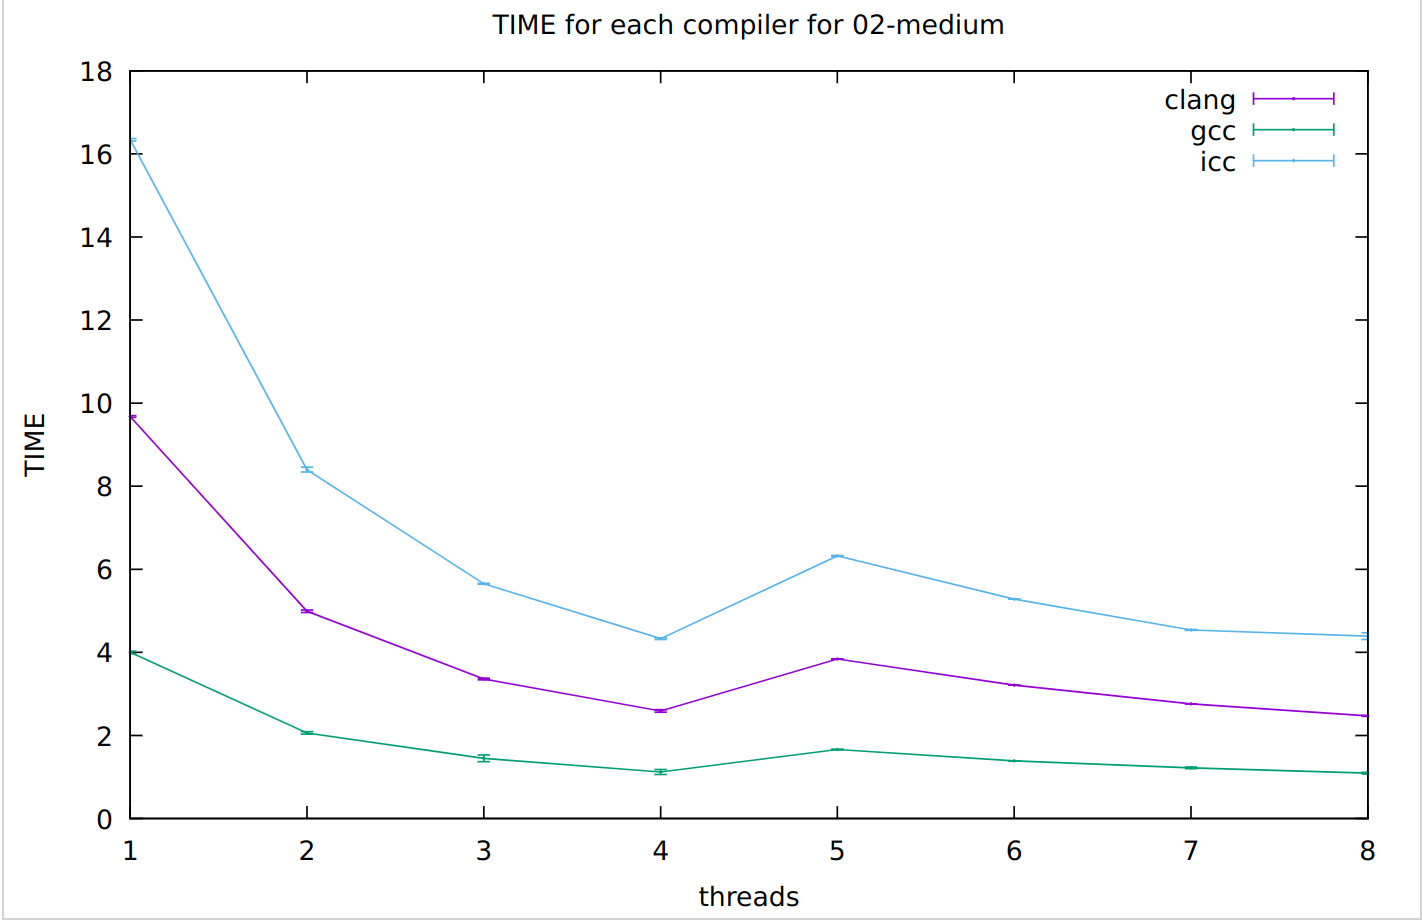
\includegraphics[width=\textwidth]{bucle2-3=02-medium}
    \end{subfigure}
    \caption{\underline{Tamaño mediano}: Tiempos de ejecución vs nº de hilos}
    \label{bucle2-3=02-medium}
\end{figure}

%%% TABLA DE TIEMPOS E IMÁGENES %%%
\begin{figure}[H]
    \centering
    \begin{subfigure}{0.4\textwidth}
        \begin{adjustbox}{width=\textwidth} 
        \begin{tabular}{|c|c|c|c|c|}
            \hline
            \rowcolor{azul} \multicolumn{2}{|c|}{}&\multicolumn{3}{c|}{\textbf{Compiler}} \\ \hline
            \rowcolor{azul} \multicolumn{2}{|c|}{}&\texttt{clang}&\texttt{gcc}&\texttt{icc}\\ \hline
            \rowcolor{azul} \textbf{Testing size} & \textbf{Threads}&\multicolumn{3}{c|}{\textbf{Average time (s)}} \\ \hline
            \multirow{8}{1cm}{\textbf{03-large}} & 1 & \(16.48\pm{0.01}\) & \(6.96\pm{0.12}\) & \(27.84\pm{0.06}\) \\ \cline{2-5}
            & 2 & \(8.54\pm{0.04}\) & \(3.55\pm{0.10}\) & \(14.33\pm{0.07}\) \\ \cline{2-5}
            & 3 & \(5.75\pm{0.00}\) & \(2.39\pm{0.03}\) & \(9.61\pm{0.06}\) \\ \cline{2-5}
            & 4 & \(4.41\pm{0.00}\) & \(1.85\pm{0.06}\) & \(7.35\pm{0.00}\) \\ \cline{2-5}
            & 5 & \(6.60\pm{0.05}\) & \(2.82\pm{0.01}\) & \(10.79\pm{0.02}\) \\ \cline{2-5}
            & 6 & \(5.48\pm{0.01}\) & \(2.36\pm{0.01}\) & \(8.99\pm{0.01}\) \\ \cline{2-5}
            & 7 & \(4.69\pm{0.02}\) & \(2.03\pm{0.01}\) & \(7.72\pm{0.00}\) \\ \cline{2-5}
            & 8 & \(4.16\pm{0.00}\) & \(1.82\pm{0.03}\) & \(6.90\pm{0.04}\) \\ \hline
        \end{tabular}
        \end{adjustbox}
    \end{subfigure}
    \hfill
    \begin{subfigure}{0.5\textwidth}
        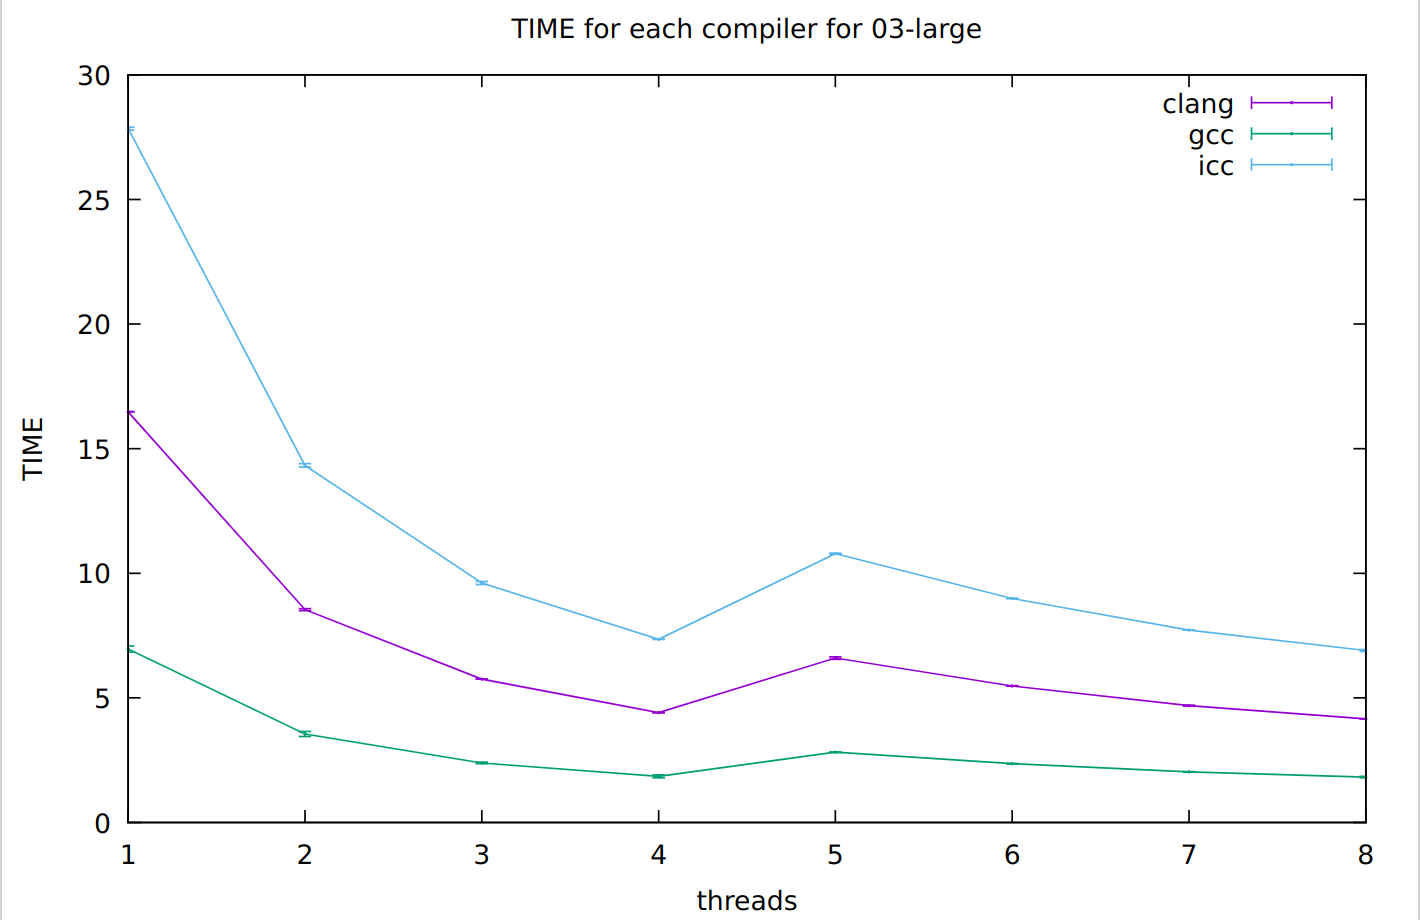
\includegraphics[width=\textwidth]{bucle2-3=03-large}
    \end{subfigure}
    \caption{\underline{Tamaño largo}: Tiempos de ejecución vs nº de hilos}
    \label{bucle2-3=03-large}
\end{figure}





\newpage